\documentclass{article}
\usepackage[a6paper, width=166pt, height=294pt]{geometry}  
\usepackage{graphicx}
\usepackage{shandean}
\usepackage{luamplib}
\title{The Life and Opinions of Tristram Shandy, Gentleman}
\author{Laurence Sterne}
\begin{document}
\pagestyle{empty}
% half title
\null
\vfill
$$\vbox{\openup 10pt\halign{\hss #\hss\cr
\hbox to 3em{T H E}\cr
\large \ls{LIFE} and \ls{OPINIONS}\cr
\hbox to 1.6em{O F}\cr
\large \ls{TRISTRAM SHANDY}, Gent.\cr
}}$$
\vfill
\newpage
\null
\newpage % full title
\vbox{\openup 10pt\halign{\hss #\hss\cr
\hbox to 3em{T H E}\cr
\lower 2pt\hbox to 9em{\Large\bfseries L I F E}\cr
\hbox to 3em{A N D}\cr
\lower 3pt\hbox to 15em{\Large\bfseries O P I N I O N S}\cr
\textsc{o f}\cr
\hbox{\large\bfseries \lsss{TRISTRAM SHANDY},}\cr
\lower-2pt\hbox{\textsc{\lss{Gentleman}.}}\cr
}}
\vfill
\vbox{\openup -2pt\halign to 180pt{\footnotesize #\cr
\textit{Dixero si quid fortè jocosius, hoc mihi juris}\hfill\cr
\textit{Cum venia dabis}.\tsh \hfill \textsc{Hor.}\cr
\noalign{\vskip 4pt}
\hbox to 1em{\tsk}\textit{Si quis calumnietur levius esse quam decet theo-}\cr
\quad\textit{logum, aut mordacius quam deceat Christianum}\cr
\quad\textit{\tsk non Ego, sed Democritus dixit}.\tsk\hfill\textsc{Erasmus}.\cr}}
\vfill
\centerline{\lsss{VOL}.\quad VI.}
\vfill
\centerline{\lsss{LONDON}:}
\centerline{\small Printed for T. \textsc{Becket} and P. A. \textsc{Dehondt},}
\centerline{\small in the Strand.\quad MDCCLXII.}

\newpage
\null
\newpage
\pagestyle{fancy}
\thispagestyle{empty}
\setcounter{page}{1}
\hbox{}\vskip -36pt
\moveright 88pt\vbox to 0pt{\hsize
40pt\rlap{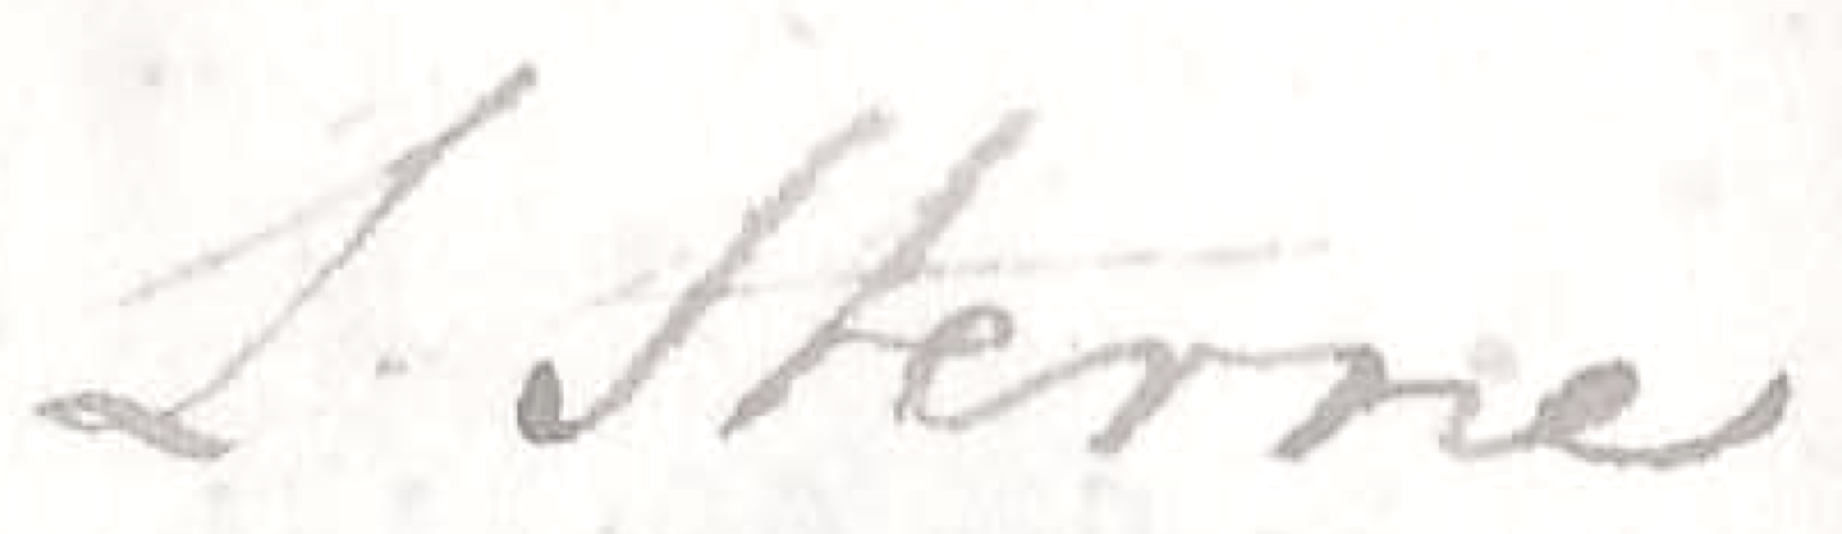
\includegraphics[width=60pt]{sterne.png}}\vss}

\[\vbox{\openup 12pt\halign{\hss # \hss\cr
\addfontfeature{LetterSpace=12.0}\textsc{the}\cr
\addfontfeature{LetterSpace=12.0}LIFE and OPINIONS\cr
\addfontfeature{LetterSpace=12.0}\textsc{of}\cr
{\addfontfeature{LetterSpace=16.0}TRISTRAM SHANDY}, Gent.\cr}}\]

\vskip 12pt
\hrule

\bigskip
\setlength{\baselineskip}{14pt}  % 21*14 = 294   294/23 \simeq 12.7826 
\sloppy

\section{\lsss{CHAP}.\enspace I.}

\lettrine{\Tsk W}{\,\ls{e’ll}} not stop two moments, my dear Sir,\tsk only, as we have got through
these five volumes, (do, Sir, sit down upon a set\tsh they are better than nothing)
let us just look back upon the country we have pass’d through.\tsh

\tsh What a wilderness has it been!\break and what a mercy
that we have not both\catch{of} of us been lost, or devoured by wild beasts
in it!

Did you think the world itself, Sir, had contained such a number
of Jack Asses?\tsh How they view’d and
review’d us as we passed over the rivulet at the bottom of
that little valley!\tsh and when we climbed over that
hill, and were just getting out of sight\tsk good God! what a
braying did they all set up together!

\tsh Prithee, shepherd! who keeps all those
Jack Asses? \quad\ast\quad\ast\quad\ast

\tsh Heaven be their comforter\tsh\break What! are
they never curried?\tsh Are they never taken in in
winter?\tsh Bray\break bray\tsk bray. Bray on,\tsk the world
is deeply your debtor;\tsh louder still\tsk\catch{that’s} that’s
nothing:\tsk in good sooth, you are ill-used:\tsh Was I
a Jack Asse, I solemnly declare, I would bray in G-sol-re-ut from
morning, even unto night.

\section{\lsss{CHAP}.\enspace II.}

\lettrine{W}{hen} my father had danced his white bear backwards and forwards through
half a dozen pages, he closed the book for good an’ all,\tsk and in a kind of
triumph redelivered it into \textit{Trim}’s hand, with a nod to lay it upon the
’scrutoire, where he found it.\tsh \textit{Tristram}, said he, shall be made to
conjugate every word in the dictionary, backwards and forwards the same way;\tsh
every word, \textit{Yorick}, by this means, you see, is converted into a thesis or
an hypothesis;\tsk every thesis and hypothesis have an off-\catch{spring} spring of
propositions;\tsk and each proposition has its own consequences and conclusions;
every one of which leads the mind on again, into fresh tracks of enquiries and
doubtings.\tsh The force of this engine, added my father, is incredible in opening a
child’s head.\tsh ’Tis enough, brother \textit{Shandy}, cried my uncle
\textit{Toby}, to burst it into a thousand\break splinters.\tsh

I presume, said \textit{Yorick}, smiling,\tsk it must be owing to
this,\tsk (for let logicians say what they will, it is not to be accounted
for sufficiently from the bare use of the ten predicaments)\tsh That
the famous \textit{Vincent Quirino}, amongst the many other astonishing feats of
his childhood, of which the Cardinal \textit{Bembo} has given the world so exact
a story,\tsk should be able to paste up in the publick schools\catch{at}
at \textit{Rome}, so early as in the eighth year of his age, no less than four
thousand, five hundred, and fifty different theses, upon the most abstruse points of
the most abstruse theology;\tsk and to defend and maintain them in such sort, as to
cramp and dumbfound his opponents.\tsh\break What is that, cried my father, to what
is told us of \textit{Alphonsus Tostatus}, who, almost in his nurse’s arms, learned
all the sciences and liberal arts without being taught any one of them?\tsh What
shall we say of the great \textit{Piereskius?}\tsk\break That’s the very man, cried
my uncle \textit{Toby}, I once told you of, brother \textit{Shandy}, who walked a
matter of five hundred miles, reckoning from \textit{Paris} to \textit{Schevling},
and from \textit{Schevling} back again, merely to see \textit{Stevinus}’s flying
chariot.\tsh He was a very great man! added my uncle \textit{Toby}; (meaning
\textit{Stevinus})\tsk He was so;\catch{bro-} brother \textit{Toby}, said my father (meaning
\textit{Piereskius})\tsk\enlargethispage\baselineskip
and had multiplied his ideas so fast, and increased his
know-\break lege to such a prodigious stock, that, if we may give credit to an anecdote
concerning him, which we cannot with-\break\tight{hold here, without shaking the
authority}
\stick{of all anecdotes whatever\tsk at seven years}
\stick{of age, his father committed entirely to}
\stick{his care the education of his younger bro-}
\stick{\tight{ther, a boy of five years old,\tsk with the sole}}
\stick{\tight{management of all his concerns.\tsk Was the}}
\stick{\tight{father as wise as the son? quoth my uncle}}
\stick{\tight{\textit{Toby}:\tsk I should think not, said \textit{Yorick}:\tsk}}
\stick{\tight{But what are these, continued my father\tsk}}
(breaking out in a kind of enthusiasm)\break
\tsk what are
these, to those prodigies of childhood in \textit{Grotius, Scioppius, Heinsius,
Politian, Pascal, Joseph Scaliger, Ferdinand de Cordouè}, and others\tsk some of
which left off their \textit{substantial forms} at\catch{nine}
nine years old, or sooner, and went on reasoning without them;\tsk others went
through their classics at seven;\tsk wrote \stick{tragedies at eight;\tsh \textit{Ferdinand
de Cor-}}\break
\stick{\textit{douè} was so wise at nine,\tsk ’twas thought}
\stick{the Devil was in him;\tsk and at \textit{Venice}}
\stick{gave such proofs of his knowledge and}
\stick{goodness, that the monks imagined he}
\stick{was \textit{Antichrist}, or nothing.\tsh Others}
\stick{were masters of fourteen languages at}
\stick{ten,\tsk finished the course of their rhe-}
toric, poetry, logic, and ethics, at eleven,\break
\tsk put forth their commentaries upon\break
\textit{Servius} and \textit{Martianus Capella} at twelve,\break
\tsk and at thirteen received their degrees in
philosophy, laws, and divinity:\tsh\break
But you forget the great \textit{Lipsius}, quoth
\textit{Yorick}, who composed a work \lower -2pt\hbox{\ast} the day\break
\rightline{he}

\vfill
\bgroup\footnotesize
\indent\fnast\ Nous aurions quelque interêt, says
\textit{Baillet}, de montrer qu’il n’a rien de ridicule s’il étoit vérita-
\break\null\hfill ble,\parfillskip0pt\par\egroup

\eject\noindent
he was born:\tsh They should have wiped it up, said my uncle
\textit{Toby}, and said no more about it.

\section{\lsss{CHAP}.\enspace III.}

\lettrine{W}{\,\ls{hen}} the cataplasm was ready, a\break
scruple of \textit{decorum} had unseas-\break onably rose up in
\textit{Susannah}’s conscience, about holding the candle,
whilst \textit{Slop} tied it on; \textit{Slop} had not treated
\textit{Susannah}’s distemper with anodines,\tsk and so a
quarrel had ensued betwixt them.

\vfill
\bgroup\footnotesize
\noindent
ble, au
moins dans le sens énigmatique que \textit{Nicius Erythræus} a tâché de lui donner.
Cet auteur dit que pour comprendre comme \textit{Lipse}, il a pû composer un ouvrage
le premier jour de sa vie, il faut s’imaginer, que ce premier jour n’est pas celui
de sa naissance charnelle, mais celui au quel il a commencé d’user de la raison; il
veut que ç’ait été à l’âge de \textit{neuf} ans; et il nous veut persuader que ce
fut en cet âge, que \textit{Lipse} fit un poëme.\tsh Le tour est ingénieux, \&c.
\&c.\par\egroup
\rightline{\tsh Oh!}
\eject

\tsh Oh! oh!\tsh said \textit{Slop},
casting a glance of undue freedom in \textit{Susannah}’s face,
as she declined the office;\tsk then,\break I think I know you,
madam\tsh You know me, Sir! cried \textit{Susannah}
fastidiously, and with a toss of her head, levelled evidently, not
at his profession, but at the doctor himself,\tsk you know\break
me! cried \textit{Susannah} again.\tsk Doctor \textit{Slop}
clapped his finger and his thumb instantly upon his
nostrils;\tsh \textit{Susannah}’s spleen was ready to
burst at it;\tsh ’Tis false, said
\textit{Susannah}.\tsk Come, come, Mrs.\@ Modesty, said \textit{Slop},
not a little\break\stick{elated with the success of his last
thrust,}\break\tsh If you won’t hold the candle, and
look\tsk you may hold it and shut your eyes:\tsk That’s
one of your popish shifts, cried \textit{Susannah:}\tsk ’Tis
better, said \textit{Slop}, with a nod, than no shift at all, young\catch{woman;}
woman;\tsh I defy you, Sir, cried \textit{Susannah}, pulling
her shift sleeve below her elbow.

It was almost impossible for two persons to assist each other in
a surgical case with a more splenetic cordiality.


\textit{Slop} snatched up the cataplasm\tsh\break
\textit{Susannah} snatched up the candle;\tsh\break
A little this way, said \textit{Slop}; \textit{Susannah}
looking one way, and rowing another, instantly set fire to \textit{Slop}’s
wig, which being somewhat bushy and unctuous withal, was burnt out before it
was well kindled.\tsh You impudent whore! cried
\textit{Slop},\tsk (for what is passion, but a wild beast)\tsk you impudent
whore, cried \textit{Slop}, getting upright, with the cataplasm in his
hand;\tsh I never was the destruction of any body’s nose, said
\textit{Susannah},\tsk which is more than you can say:\catch{\tsh Is} \tsh Is it?
cried \textit{Slop}, throwing the cataplasm in her face;\tsh Yes, it is,
cried \textit{Susannah}, returning the compliment with what was left in the pan.\tsh

\vskip -6pt

\section{\lsss{CHAP}.\enspace IV.}

\lettrine{D}{octor} \textit{Slop} and
\textit{Susannah} filed cross-bills against each other in the
parlour; which done, as the cataplasm had failed, they retired into
the kitchen to prepare a fomentation for me;\tsk and whilst that was doing, my father determined the
point as you will read.

\vskip -6pt
\enlargethispage\baselineskip

\section{\lsss{CHAP}.\enspace V.}

\lettrine{Y}{ou} see ’tis high time, said my
father, addressing himself equally to my uncle \textit{Toby} and
\textit{Yorick}, to take this young creature out of these
women’s hands, and put him into those of a private governor.
\textit{Marcus Antoninus} provided four-\catch{teen} teen governors all at once to
superintend his son \textit{Commodus}’s education,\tsk and in
six weeks he cashiered five of them;\tsk \break I know very well,
continued my father, that \textit{Commodus}’s mother was in
love with a gladiator at the time of her conception, which accounts
for a great many of \textit{Commodus}’s cruelties when he
became emperor;\tsk but still I am of opinion, that those five
whom \textit{Antoninus} dismissed, did \textit{Commodus}’s
temper, in that short time, more hurt than the other nine were able
to rectify all their lives long.

Now as I consider the person who is to be about my son, as the
mirror in which he is to view himself from morning to night,
by which he is to adjust his looks, his carriage, and perhaps the
inmost sentiments of his heart;\tsk I would have one,
\textit{Yorick}, if possible, polished at\catch{all} all points, fit for my
child to look into.\break\tsh This is very good sense, quoth my
uncle \textit{Toby} to himself.

\tsh There is, continued my father, a certain mien and
motion of the body and all its parts, both in acting and speaking,
which argues a man \textit{well within}; and I am not at all
surprised that \textit{Gregory} of \textit{Nazianzum}, upon observing
the hasty and untoward gestures of \textit{Julian}, should foretel he
would one day become an apostate;\tsh or that St.\@ \textit{Ambrose} should turn his \textit{Amanuensis} out of doors,
because of an indecent motion of his head, which went backwards and
forwards like a flail;\tsh or that \textit{Democritus}
should conceive \textit{Protagoras} to be a scholar, from seeing him
bind up a faggot, and thrusting, as he did it, the small twigs
inwards.\tsh There are a\catch{thou-} thousand unnoticed openings,
continued my father, which let a penetrating eye at once into
a man’s soul; and I maintain it, added he, that a man of
sense does not lay down his hat in coming into a room,\tsk or
take it up in going out of it, but something escapes, which
discovers him.

It is for these reasons, continued my father, that the governor
I make choice of shall neither \fnast\ lisp, or squint, or
wink,\break or talk loud, or look fierce, or foolish;\break\tsh
or bite his lips, or grind his teeth, or speak through his nose,
or pick it, or blow it with his fingers.\tsh

He shall neither walk fast,\tsk or slow, or fold his
arms,\tsk for that is laziness; \tsk\break or hang them
down,\tsk for that is folly;\break
\centerline{\footnotesize \fnast\ Vid. \textit{Pellegrina}.}
\rightline{or}
\eject
\noindent
or hide them in his pocket, for that is nonsense.\tsh

He shall neither strike, or pinch, or tickle\tsk or bite, or
cut his nails, or hawk, or spit, or snift, or drum with his feet or
fingers in company;\tsh nor (according to \textit{Erasmus})
shall he speak to any one in making water,\tsk nor shall he point to
carrion or excrement.\tsh Now this is all nonsense again,
quoth my uncle \textit{Toby} to himself.\tsh

I will have him, continued my father, cheerful, faceté,
jovial; at the same time, prudent, attentive to business, vigilant,
acute, argute, inventive, quick in resolving doubts and speculative
questions;\tsh he shall be wise, and judicious, and
learned:\tsh And why not humble, and moderate, and
gentle-tempered, and\catch{good?} good? said \textit{Yorick}:\tsh And why
not, cried my uncle \textit{Toby}, free, and generous, and bountiful,
and brave?\tsh He shall, my dear \textit{Toby}, replied my
father, getting up and shaking him by his hand.\tsk Then, brother
\textit{Shandy}, answered my uncle \textit{Toby}, raising himself off
the chair, and laying down his pipe to take hold of my
father’s other hand,\tsk I humbly beg I may recommend poor
\textit{Le Fever}’s son to you;\tsh a tear of joy of
the first water sparkled in my uncle \textit{Toby}’s eye, and
another, the fellow to it, in the corporal’s, as the
proposition was made;\tsh you will see why when you read \textit{Le
Fever}’s story:\tsh fool that I was! nor can I
recollect (nor perhaps you) without turning back to the place, what
it was that hindered me from letting the corporal tell it in his
own words;\tsk but\catch{the} the occasion is lost,\tsk I must tell it now
in my own.






\section{\lsss{CHAP}.\enspace VI.}

\medskip
\centerline{\textit{The Story of} \textsc{Le Fever}.}

\lettrine{I}{t} was some time in the summer of
that year in which \textit{Dendermond} was taken by the
allies,\tsk which was about seven years before my father came
into the country,\tsk and about as many, after the time, that my
uncle \textit{Toby} and \textit{Trim} had privately decamped from my
father’s house in town, in order to lay some of the finest
sieges to some of the finest fortified cities in
\textit{Europe}\tsh when my uncle \textit{Toby} was one
evening getting his supper, with \textit{Trim} sitting behind him at
a small sideboard,\tsk I say, sitting\tsk for\catch{in}
in consideration of the corporal’s lame knee
(which sometimes gave him exqui\-site pain)\tsk when my uncle
\textit{Toby} dined or supped alone, he would never suffer the
corporal to stand; and the poor fellow’s veneration for his
master was such, that, with a proper artillery, my uncle
\textit{Toby} could have taken \textit{Dendermond} itself, with less
trouble than he was able to gain this point over him; for many a
time when my uncle \textit{Toby} supposed the corporal’s leg
was at rest, he would look back, and detect him standing behind him
with the most dutiful respect: this bred more little squabbles
betwixt them, than all other causes for five-and-twenty years
together\tsk But this is neither here nor there\tsk why do I
mention it?\tsh\break Ask my pen,\tsk it governs me,\tsk I
govern not it.\patch{He}

He was one evening sitting thus at his supper, when the landlord
of a little inn in the village came into the parlour, with an
empty phial in his hand, to beg a glass or two of sack; ’Tis for
a poor gentleman,\tsk I think, of the army, said the landlord,
who has been taken ill at my house four days ago, and has never
held up his head since, or had a desire to taste any thing, till
just now, that he has a fancy for a glass of sack and a thin
toast,\tsh \textit{I~think}, says he, taking his hand from his
forehead, \textit{it would comfort me.}\tsh

\tsh If I could neither beg, borrow, or buy such a thing\tsk
added the landlord,\tsk I~would almost steal it for the poor
gentleman, he is so ill.\tsh I hope in God he will still mend,
continued he,\tsk we are all of us concerned for him.\patch{Thou}

Thou art a good-natured soul, I will answer for thee, cried my
uncle \textit{Toby}; and thou shalt drink the poor gentleman’s
health in a glass of sack thyself,\break\tsk and take a couple of
bottles with my service, and tell him he is heartily welcome to
them, and to a dozen more if they will do him good.

Though I am persuaded, said my uncle \textit{Toby}, as the
landlord shut the door, he is a very compassionate
fellow\tsk \textit{Trim},\break\tsk yet I cannot help entertaining a high opinion
of his guest too; there must be something more than common in him,
that in so short a time should win so much upon the affections of
his host;\tsh And of his whole family, added the corporal,
for they are all concerned for him.\tsh Step after him,
said my\catch{uncle} uncle \textit{Toby},\tsk do \textit{Trim},\tsk and ask if
he knows his name.

\tsh I have quite forgot it truly, said the landlord,
coming back into the parlour with the corporal,\tsk but I can ask
his son again:\tsh Has he a son with him then? said my
uncle \textit{Toby}.\tsk A boy,\break replied the landlord, of about
eleven or twelve years of age;\tsk but the poor creature has
tasted almost as little as his father; he does nothing but mourn
and lament for him night and day:\tsh He has not stirred
from the bed-side these two days.

My uncle \textit{Toby} laid down his knife and fork, and thrust
his plate from before him, as the landlord gave him the account;
and \textit{Trim}, without being ordered, took away, without
saying one\catch{word,} word, and in a few minutes after brought him his
pipe and tobacco.

\tsh Stay in the room a little, said my uncle
\textit{Toby}.\tsh

\textit{Trim!}\tsh said my uncle \textit{Toby}, after
he lighted his pipe, and smoak’d about a dozen
whiffs.\tsh \textit{Trim} came in front of his master, and
made his bow;\tsk my uncle \textit{Toby} smoak’d on, and said
no more.\tsh Corporal! said my uncle \textit{Toby}\break\tsh the
corporal made his bow.\tsh\break My uncle \textit{Toby} proceeded
no farther, but finished his pipe.

\textit{Trim!} said my uncle \textit{Toby}, I have a project
in my head, as it is a bad night, of wrapping myself up warm in my
roquelaure, and paying a visit to this poor
gentleman.\tsh Your honour’s roque-\catch{laure,} laure, replied the
corporal, has not once been had on, since the night before your
honour received your wound, when we mounted guard in the trenches
before the gate of St.~\textit{Nicholas};\tsk and besides, it is so
cold and rainy a night, that what with the roquelaure, and what with the
weather, ’twill be enough to give your honour your death, and
bring on your honour’s torment in your groin. I fear so,
replied my uncle \textit{Toby}; but I am not at rest in my mind,
\textit{Trim}, since the account the landlord has given
me.\tsh I wish I had not known so much of this
affair,\tsk added my uncle \textit{Toby},\tsk or that I had known
more of it:\tsh How shall we manage it? Leave it,
an’t please your honour, to me, quoth the
corporal;\tsh I’ll take my hat and stick and go to
the house and reconnoitre, and act accordingly; and I will bring
your\catch{honour}
honour a full account in an hour.\tsh\break
Thou shalt go, \textit{Trim}, said my uncle \textit{Toby}, and
here’s a shilling for thee to drink with his servant.\tsh I
shall get it all out of him, said the corporal, shutting the
door.

My uncle \textit{Toby} filled his second pipe; and had it not
been, that he now and then wandered from the point, with
considering whether it was not full as well to have the curtain of the tennaile a straight
line, as a crooked one,\tsk he might be said to have thought of
nothing else but poor \textit{Le Fever} and his boy the whole time he
smoaked it.

\vfill\rightline{\ls{CHAP}.}\eject
\section{\lsss{CHAP}.\enspace VII.}

\medskip
\centerline{\textit{The Story of} \textsc{Le Fever} \textit{continued}.}

\lettrine It was not till my uncle \textit{Toby} had knocked the
ashes out of his third pipe, that corporal \textit{Trim}
returned from the inn, and gave him the following\break account.

I despaired, at first, said the corporal, of being able to bring
back your honour any kind of intelligence concerning the poor
sick lieutenant\tsk Is he in the army, then? said my uncle
\textit{Toby}\tsh He is, said the corporal\tsh And in what
regiment? said my uncle \textit{Toby}\tsh I’ll tell your honour,
replied the corporal, every thing straight forwards, as I learnt
it.\tsk\break Then, \textit{Trim}, I’ll fill another pipe, said my
uncle \textit{Toby}, and not interrupt thee\catch{till}
till thou hast done; so sit down at thy ease, \textit{Trim}, in
the window seat, and begin thy story again. The corporal made
his old bow, which generally spoke as plain as a bow could speak
it\tsk \textit{Your\break honour is good}:\tsk And having done that,
he sat down, as he was ordered,\tsk\break and begun the story to my
uncle \textit{Toby} over again in pretty near the same\break words.

I despaired at first, said the corporal, of being able to bring
back any intelligence to your honour, about the lieutenant and his
son; for when I asked where his servant was, from whom I made
myself sure of knowing every thing which was proper to be
asked,\tsk\break That’s a right distinction, \textit{Trim}, said my
uncle \textit{Toby}\tsk I was answered, an’ please your
honour, that he had no servant\catch{with} with him;\tsh that he had
come to the inn with hired horses, which, upon finding himself
unable to proceed (to join, I suppose, the regiment), he had
dismissed the morning after he came.\tsk If I get better, my
dear, said he, as he gave his purse to his son to pay the man,\tsk we
can hire horses from hence.\tsh But alas! the poor
gentleman will never get from hence, said the landlady to
me,\tsk for I heard the death-watch all night
long;\tsh and when he dies, the youth, his son, will
certainly die with him; for he is broken-hearted already.

I was hearing this account, continued the corporal, when the
youth came into the kitchen, to order the thin toast the landlord
spoke of;\tsh but I will do it for my father myself, said
the youth.\break\tsh Pray let my save you the trouble,\catch{young}
young gentleman, said I, taking up a fork for the purpose, and
offering him my chair to sit down upon by the fire, whilst I did
it.\tsh I believe, Sir, said he, very modestly, I can please him
best myself.\tsh I am sure, said I, his honour will not like the
toast the worse for being toasted by an old soldier.\tsh The
youth took hold of my hand, and instantly burst into tears.\tsh
Poor youth! said my uncle \textit{Toby},\tsk he has been bred up
from an infant in the army, and the name of a soldier,
\textit{Trim}, sounded in his ears like the name of a
friend;\tsk I wish I had him here.

\tsh I never, in the longest march, said the corporal,
had so great a mind to my dinner, as I had to cry with him for
company:\tsk What could be the matter with me, an’ please
your honour?\catch{Nothing} Nothing in the world, \textit{Trim}, said my uncle
\textit{Toby}, blowing his nose,\tsk but that thou art a
good-natured fellow.

When I gave him the toast, continued the corporal, I thought it
was proper to tell him I was Captain \textit{Shandy}’s servant,
and that your honour (though a stranger) was extremely concerned
for his father;\tsk and that if there was any thing in your house
or cellar\tsh (And thou might’st have added my purse
too, said my uncle \textit{Toby})\tsh he was heartily
welcome to it:\tsh He made a very low bow, (which was meant
to your honour) but no answer\tsk for his heart was
full\tsk\break so he went up stairs with the toast;\tsk I warrant
you, my dear, said I, as I opened the kitchen-door, your father
will be well again.\tsh Mr.\@ \textit{Yorick}’s
curate was\catch{smoak-} smoaking a pipe by the kitchen fire,\tsk but said not a
word good or bad to comfort the youth.\tsh I thought it
wrong; added the corporal\tsh I think so too, said my
uncle \textit{Toby.}

When the lieutenant had taken his glass of sack and toast, he
felt himself a little revived, and sent down into the kitchen, to
let me know, that in about\break
ten minutes he should be glad if I would
step up stairs.\tsh I believe, said the landlord, he is
going to say his prayers,\tsh for there was a book laid
upon the chair by his bedside, and as I shut the door, I saw his
son take up a\break cushion.\tsh

I thought, said the curate, that you gentlemen of the army, Mr.
\textit{Trim}, never said your prayers at all.\tsh I heard
the\catch{poor} poor gentleman say his prayers last night, said the landlady,
very devoutly, and with my own ears, or I could not have believed
it.\tsh Are you sure of it? replied the
curate.\tsh A soldier, an’ please your reverence,
said I, prays as often (of his own accord) as a
parson;\break\tsh and when he is fighting for his king, and for
his own life, and for his honour too, he has the most reason to
pray to God of any one in the whole world\tsh ’Twas
well said of thee, \textit{Trim}, said my uncle
\textit{Toby.}\tsh But when a soldier, said I, an’
please your reverence, has been standing for twelve hours together
in the trenches, up to his knees in cold water,\tsk or engaged,
said I, for months together in long and dangerous
marches;\tsk harassed, perhaps, in his\break rear
to-day;\tsk harassing others to-mor-\break row;\tsk detached
here;\tsk countermanded\catch{there;} there;\tsk resting this night out upon
his arms;\tsk beat up in his shirt the next;\tsk benumbed in
his joints;\tsk perhaps without straw in his tent to kneel
on;\tsk must say his prayers \textit{how} and \textit{when} he
can.\tsk I believe, said I,\tsk for I was piqued, quoth the
corporal, for the reputation of the army,\tsk I believe,
an’ please your reverence, said I, that when a soldier gets
time to pray,\tsk he prays as heartily as a parson,\tsk though
not with all his fuss and hypocrisy.\tsh Thou shouldst not
have said that, \textit{Trim}, said my uncle \textit{Toby},\tsk for
God only knows who is a hypocrite, and who is not:\tsh At
the great and general review of us all, corporal, at the day of
judgment (and not till then)\tsk it will be seen who has done
their duties in this world,\tsk and who has not; and we shall be
advanced, \textit{Trim}, accordingly.\tsh I hope we shall,\catch{said}
said \textit{Trim.}\tsh It is in the Scripture, said my
uncle \textit{Toby}; and I will shew it thee to-morrow:\tsh In the
mean time we may depend upon it, \textit{Trim}, for our comfort, said
my uncle \textit{Toby}, that God Almighty is so good and just a
governor of the world, that if we have but done our duties in
it,\tsh it will never be enquired into, whether we have done them
in a red coat or a black one:\tsh\break I hope not, said the
corporal\tsh But go on, \textit{Trim}, said my uncle
\textit{Toby}, with\break thy story.

When I went up, continued the corporal, into the
lieutenant’s room, which I did not do till the expiration of
the ten minutes,\tsk he was lying in his bed with his
head raised upon his hand, with his elbow upon the pillow, and a
clean white cambrick handkerchief be-\catch{side} side it:\tsh The youth
was just stooping down to take up the cushion, upon which I
supposed he had been kneeling,\tsk the book was laid upon the
bed,\tsk and, as he rose, in taking up the cushion with one hand,
he reached out his other to take it away at the same
time.\tsh Let it remain there, my dear, said the
lieutenant.

He did not offer to speak to me, till I had walked up close to
his bed- side:\tsk If you are captain \textit{Shandy}’s
servant, said he, you must present my thanks to your master, with
my little boy’s thanks along with them, for his courtesy to
me;\tsk if he was of \textit{Levens}’s\tsk said the
lieutenant.\tsk I told him your honour was\tsk Then, said he, I
served three campaigns with him in \textit{Flanders}, and remember
him,\tsk but ’tis most likely, as\catch{I had} I had not the honour of
any acquaintance with him, that he knows nothing of me.\tsh You will tell him, however, that
the person his good-nature has laid under obligations to him, is
one \textit{Le Fever}, a lieutenant in
\textit{Angus}’s\tsh but he knows me not,\tsk said
he, a second time, musing;\tsh possibly he may my
story\tsk added he\tsk pray tell the captain, I was the ensign
at \textit{Breda}, whose wife was most unfortunately killed with a
musket-shot, as she lay in my arms in my tent.\tsh I
remember the story, an’t please your honour, said I, very
well.\tsh Do you so? said he, wiping his eyes with his
handkerchief\tsk then well may I.\tsk In saying this, he drew a
little ring out of his bosom, which seemed tied with a black
ribband about his neck, and kiss’d it
twice\tsh Here, \textit{Billy}, said he,\tsk the boy flew
across the room to\catch{the} the bed-side,\tsk and falling down upon his
knee, took the ring in his hand, and kissed it too,\tsk then
kissed his father, and sat down upon the bed and wept.

I wish, said my uncle \textit{Toby}, with a deep sigh,\tsk I
wish, \textit{Trim}, I was asleep.

Your honour, replied the corporal, is too much
concerned;\tsk shall I pour your honour out a glass of sack to
your pipe?\tsh Do, \textit{Trim}, said my uncle
\textit{Toby.}

I remember, said my uncle \textit{Toby}, sighing again, the story
of the ensign and his wife, with a circumstance his modesty
omitted;\tsk and particularly well that he, as well as she, upon
some account or other (I forget what) was universally pitied by the
whole regiment;\catch{\tsk but} \tsk but finish the story thou art
upon:\break\tsk ’Tis finished already, said the
corporal,\tsk for I could stay no longer,\tsk so wished his
honour a good night; young \textit{Le Fever} rose from off the bed,
and saw me to the bottom of the stairs; and as we went down
together, told me, they had come from \textit{Ireland}, and were on
their route to join the regiment in
\textit{Flanders.}\tsh But alas! said the
corporal,\tsk the lieutenant’s last day’s march is
over.\tsk Then what is to become of his poor boy? cried my uncle
\textit{Toby.}

\section{\lsss{CHAP}.\enspace VIII.}
\centerline{\textit{The Story of} \textsc{Le Fever} \textit{continued}.}

\lettrine{I}{\,t} was to my uncle
\textit{Toby}’s eternal honour,\tsh though I tell it
only for the sake of those, who, when coop’d in betwixt a
natural and a positive law,\catch{know} know not for their souls, which way in
the world to turn themselves\tsk That\break\stick{\tight{notwithstanding my
uncle \textit{Toby} was warm}-}\break ly engaged at that time in carrying on
the siege of \textit{Dendermond}, parallel with the allies, who
pressed theirs on so vigorously, that they scarce allowed him time
to get his dinner\tsh that nevertheless he gave up
\textit{Dendermond}, though he had already made a lodgment upon the
counterscarp;\tsh and bent his whole thoughts towards the private
distresses at the inn; and except that he ordered the garden gate
to be bolted up, by which he might be said to have turned the siege
of \textit{Dendermond} into a blockade,\tsk he left
\textit{Dendermond} to itself,\tsk to be relieved or not by the \textit{French} king, as the
\textit{French} king thought good; and only considered how he himself
should relieve the poor lieutenant and his son.\etp\patch{\tsh That}

\tsh That kind \textsc{Being}, who is a friend to
the friendless, shall recompence thee for this.

Thou hast left this matter short, said my uncle \textit{Toby} to
the corporal, as he was putting him to bed,\tsh and I will
tell thee in what, \textit{Trim.}\tsh In the first place,
when thou madest an offer of my services to \textit{Le
Fever},\tsh as sickness and travelling are both
expensive, and thou knowest he was but a poor lieutenant, with a
son to subsist as well as himself out of his pay,\tsk that thou
didst not make an offer to him of my purse; because, had he stood
in need, thou knowest, \textit{Trim}, he had been as welcome to it as
myself.\tsh Your honour knows, said the corporal, I had no
orders;\tsh True, quoth my uncle \textit{Toby},\tsk thou
didst very\catch{right,} right, \textit{Trim}, as a soldier,\tsk but certainly
very wrong as a man.

In the second place, for which, indeed, thou hast the same
excuse, continued my uncle \textit{Toby},\tsh when thou
offeredst him whatever was in my house,\tsk thou shouldst
have offered him my house too:\break\tsh A sick brother officer
should have the best quarters, \textit{Trim}, and if we had him with
us,\tsk we could tend and look to him:\tsh Thou art an
excellent nurse thyself, \textit{Trim},\tsk and what with thy care
of him, and the old woman’s and his boy’s, and mine
together, we might recruit him again at once, and set him upon his
legs.\tsh

\tsh In a fortnight or three weeks, added my uncle
\textit{Toby}, smiling,\tsh he might march.\tsh He
will never march,\catch{an’} an’ please your honour, in this world, said
the corporal:\tsh He will march; said my uncle
\textit{Toby}, rising up from the side of the bed, with one shoe
off:\tsh\break
An’ please your honour, said the corporal,
he will never march but to his grave:\tsh He shall march,
cried my uncle \textit{Toby}, marching the foot which had a shoe on,
though without advancing an inch,\tsk he shall march to his
regiment.\tsh He cannot stand it, said the
corporal;\tsh He shall be supported, said my uncle
\textit{Toby};\tsh He’ll drop at last, said the
corporal, and what will become of his boy?\tsh He shall
not drop, said my uncle \textit{Toby},
firmly.\tsh A-well-o’day,\break\tsk do what we can for
him, said \textit{Trim}, maintaining his point,\tsk the poor soul
will die:\tsh He shall not die, by G\tsk , cried my
uncle \textit{Toby.}\patch{\tsk The}

\tsk The \textsc{accusing spirit}, which flew up to
heaven’s chancery with the oath, blush’d as he gave it
in;\tsk and the \textsc{recording angel}, as he wrote it
down, dropp’d a tear upon the word, and blotted it out for
ever.

\section{\lsss{CHAP}.\enspace IX.}

\lettrine{\Tsk M}{y} uncle \textit{Toby}
went to his bureau,\tsk put his purse into his breeches pocket,
and having ordered the corporal to go early in the morning for a
physician,\tsk he went to bed, and fell asleep.

\vfill\rightline{\ls{CHAP}.}\eject
\null\par
\section{\lsss{CHAP}.\enspace X.}

\smallskip
\centerline{\textit{The Story of} \textsc{Le Fever} \textit{concluded}.}

\lettrine{T}{\,\ls{he}} sun looked bright the morning
after, to every eye in the village but \textit{Le Fever}’s and
his afflicted son’s; the hand of death pressed heavy upon his
eye-lids,\tsh and hardly could the wheel at the cistern
turn round its circle,\tsk when my uncle \textit{Toby}, who had
rose up an hour before his wonted time, entered the
lieutenant’s room, and without preface or apology, sat
himself down upon the chair by the bed-side, and, independently of
all modes and customs, opened the curtain in the manner an old
friend and brother officer would have done it, and asked him how he
did,\tsk how he had rested in the night,\tsk what\catch{was} was his
complaint,\tsk where was his pain,\tsk and what he could do to
help him:\tsh and without giving him time to answer any
one of the enquiries, went on, and told him of the little plan
which he had been concerting with the corporal the night
before for him.\tsh

\tsh You shall go home directly, \textit{Le Fever}, said
my uncle \textit{Toby}, to my house,\break\tsk and we’ll send for a
doctor to see what’s the matter,\tsk and we’ll have
an apothecary,\tsk and the corporal shall be your
nurse;\tsh and I’ll be your servant, \textit{Le
Fever}.

There was a frankness in my uncle \textit{Toby},\tsk not the
\textit{effect} of familiarity,\tsk but the \textit{cause} of
it,\tsk which let you at once into his soul, and shewed you the
goodness of his nature; to this there was\catch{some-} something in his looks,
and voice, and manner, superadded, which eternally beckoned to the
unfortunate to come and take shelter under him, so that before my
uncle \textit{Toby} had half finished the kind offers he was making
to the father, had the son insensibly pressed up close to his
knees, and had taken hold of the breast of his coat, and was
pulling it towards him.\tsh The blood and spirits of \textit{Le
Fever}, which were waxing cold and slow within him, and were
retreating to their last citadel, the heart\tsk rallied
back,\tsk the film forsook his eyes for a moment,\tsk he looked
up wishfully in my uncle \textit{Toby}’s face,\tsk then cast
a look upon his boy,\tsh and that \textit{ligament}, fine as
it was,\tsk was never broken.\tsh

Nature instantly ebb’d again,\tsk the film returned to
its place,\tsh the pulse\catch{flut-}
fluttered\tsh stopp’d\tsh went on\tsh\break
\tsh throb’d\tsh stopp’d again\tsh moved\tsh stopp’d\tsh shall
I go on?\tsh\break
No.

\section{\lsss{CHAP}.\enspace XI.}

\lettrine{I}{ am} so impatient to return to my own
story, that what remains of young\break\textit{Le Fever}’s, that is,
from this turn of his fortune, to the time my uncle \textit{Toby}
recommended him for my preceptor, shall be told in a very few words
in the next chapter.\tsk All that is necessary to be added to
this chapter is as follows.\tsk 

That my uncle \textit{Toby}, with young \textit{Le Fever} in his
hand, attended the poor\break lieutenant, as chief mourners, to his\break
grave.\patch{That}

\noindent\stick{\hfill That the governor of \textit{Dendermond} paid}
his obsequies all
military honours,\tsk and that \textit{Yorick}, not to be
behind-hand\tsk\break
paid him all ecclesiastic\tsk for he buried him
in his chancel:\tsk And it appears likewise, he preached a
funeral sermon over him\tsh I say it
\textit{appears},\tsk for it was \textit{Yorick}’s custom,
which I suppose a general one with those of his profession, on the
first leaf of every sermon which he composed, to chronicle down the
time, the place, and the occasion of its being preached: to this,
he was ever wont to add some short comment or stricture upon the
sermon itself, seldom, indeed, much to its credit:\tsk For
instance, \textit{This sermon upon the jewish dispensation\tsk I
don’t like it at all;\tsk Though I own there is a world
of} \textsc{water-landish} \textit{knowledge in it;\tsk but
’tis all tritical, and\catch{most} most tritically put
together.\tsk This is but a flimsy kind of a composition; what
was in my head when I made it?}

\tsh N.B. \textit{The excellency of this text is, that it
will suit any sermon,\tsk and of this sermon,\tsh that
it will suit any text.\tsh}

\tsh \textit{For this sermon I shall be
hanged,\break\tsk for I have stolen the greatest part of it. Doctor}
Paidagunes \textit{found me out. ☞  Set a thief to catch a
thief.\tsh}

On the back of half a dozen I find written, \textit{So}, \textit{so}, and no
more\tsh and upon a couple \textit{Moderato}; by which, as
far as one may gather from \textit{Altieri’s Italian}
dictionary,\tsk but mostly from the authority of a piece of green
whipcord, which seemed to have been the unravel-\catch{ling} ling of
\textit{Yorick}’s whip-lash, with which he has left us the two
sermons marked \textit{Moderato}, and the half dozen of \textit{So,
so}, tied fast together in one bundle by themselves,\tsk one
may safely suppose he meant pretty near the same thing.

There is but one difficulty in the way of this conjecture, which
is this, that the \textit{moderato}’s are five times better
than the \textit{so, so}’s;\tsk show ten times more knowledge
of the human heart;\tsk have seventy times more wit and spirit in
them;\tsk (and, to rise properly in my climax)\tsk discover a
thousand times more genius;\break\tsk and to crown all, are infinitely
more entertaining than those tied up with them:\tsk for
which reason, whene’er \textit{Yorick’s dramatic} sermons
are offered to the world, though I shall admit but one out of the
whole number of the \textit{so, so}’s, I shall,\catch{never-} nevertheless,
adventure to print the two \textit{moderato}’s without any sort
of scruple.

What \textit{Yorick} could mean by the words
\textit{lentamente,\tsk tenutè,\tsk grave},\tsk and
sometimes \textit{adagio},\tsk as applied to \textit{theological}
compositions, and with which he has characterised some of these
sermons, I dare not venture to guess.\tsh I am more
puzzled still upon finding \textit{a l’octava alta!} upon
one;\tsh \textit{Con strepito} upon the back of
another;\tsh \textit{Scicilliana} upon a
third;\tsh \textit{Alla capella} upon a
fourth;\tsh \textit{Con l’arco} upon
this;\tsh \textit{Senza l’arco} upon
that.\tsh All I know is, that they are musical terms, and
have a meaning;\tsh and as he was a musical man, I will
make no doubt, but that by some quaint application of such
metaphors to the compositions in hand, they impressed very distinct
ideas of their several cha-\catch{racters} racters upon his fancy,\tsk whatever
they may do upon that of others.

Amongst these, there is that particular sermon which has
unaccountably led me into this digression\tsh The funeral
sermon upon poor \textit{Le Fever}, wrote out very fairly, as if from
a hasty copy.\tsk I take notice of it the more, because it seems
to have been his favourite composition\tsh It is upon
mortality; and is tied length-ways and cross-ways with a yarn
thrum, and then rolled up and twisted round with a half-sheet of
dirty blue paper, which seems to have been once the cast cover of a
general review, which to this day smells horribly of horse
drugs.\tsh Whether these marks of humiliation were
designed,\tsk I something doubt;\tsh because at the end
of the sermon (and not at the beginning\catch{of} of it)\tsk very different
from his way of treating the rest, he had wrote\tsh

\centerline{Bravo!}
\vskip-\parskip

\tsh Though not very offensively,\break\tsh for it
is at two inches, at least, and a half’s distance from, and
below the concluding line of the sermon, at the very extremity of
the page, and in that right hand corner of it, which, you know, is
generally covered with your thumb; and, to do it justice, it is
wrote besides with a crow’s quill so faintly in a small
\textit{Italian} hand, as scarce to sollicit the eye towards the
place, whether your thumb is there or not,\tsk so that from the
\textit{manner of it}, it stands half excused; and being wrote
moreover with very pale ink, diluted almost to
nothing,\tsk ’tis more like a \textit{ritratto} of the shadow
of vanity, than of \textsc{Vanity} herself\tsk of the two;
resembling rather a faint thought\catch{of} of transient applause, secretly
stirring up in the heart of the composer; than a gross mark of it,
coarsely obtruded upon the world.

With all these extenuations, I am aware, that in publishing
this, I do no service to \textit{Yorick}’s character as a
modest man;\tsk but all men have their failings! and what lessens
this still farther, and almost wipes it away, is this; that the
word was struck through sometime afterwards (as appears from a
different tint of the ink) with a line quite across it in this manner,
\hbox to 33pt{\rlap{\,BRAVO}\leaders\hrule width 1pt height 3.4pt depth -3.1pt\hfill}\tsh as if he had retracted, or was
ashamed of the opinion he had once entertained of it.

These short characters of his sermons were always written,
excepting in this one instance, upon the first leaf of his\catch{sermon,} sermon,
which served as a cover to it; and usually upon the inside of it,
which was turned towards the text;\tsk but at the end of his
discourse, where, perhaps, he had five or six pages, and sometimes,
perhaps, a whole score to turn himself in,\tsk he took a large
circuit, and, indeed, a much more mettlesome one;\tsk as if he
had snatched the occasion of unlacing himself with a few more
frolicksome strokes at vice, than the straitness of the pulpit
allowed.\tsk These, though hussar-like, they skirmish lightly and
out of all order, are still auxiliaries on the side of
virtue;\tsk tell me then, Mynheer Vander
Blonederdondergewdenstronke, why they should not be printed
together?

\vfill\rightline{\ls{CHAP}.}\eject
\section{\lsss{CHAP}.\enspace XII.}

\lettrine{W}{\,\ls{hen}} my uncle \textit{Toby} had turned
every thing into money, and\break settled all accounts betwixt the agent
of the regiment and \textit{Le Fever}, and betwixt \textit{Le Fever}
and all mankind,\tsh\break
there remained nothing more in my uncle \textit{Toby}’s hands, than an old
regimental coat and a sword; so that my uncle \textit{Toby} found little or no
opposition from the world in taking administration. The coat my uncle \textit{Toby}
gave the corporal;\break
\tsh Wear it, \textit{Trim}, said my uncle \textit{Toby}, as long
as it will hold together, for the sake of the poor lieutenant\tsh And this,\tsh said
my uncle \textit{Toby}, taking up the sword in his hand, and drawing it out of the
scabbard as he spoke\tsk and\break this, \textit{Le Fever}, I’ll save for thee,\tsk
’tis\catch{all} all the fortune, continued my uncle \textit{Toby}, hanging it up upon a
crook, and pointing to it,\tsk ’tis all the fortune, my dear \textit{Le Fever},
which God has left thee; but if he has given thee a heart to fight thy way with it
in the world,\tsk and thou doest it like a man of honour,\tsk ’tis enough for us.

As soon as my uncle \textit{Toby} had laid a foundation, and
taught him to inscribe a regular polygon in a circle, he sent him
to a public school, where, excepting \textit{Whitsontide} and
\textit{Christmas}, at which times the corporal was punctually
dispatched for him,\tsk he remained to the spring of the year,
seventeen; when the stories of the emperor’s sending his army
into \textit{Hungary} against the \textit{Turks}, kindling a spark of
fire in his bosom, he left his \textit{Greek} and \textit{Latin}
without leave, and\catch{throw-} throwing himself upon his knees before my uncle
\textit{Toby}, begged his father’s sword, and my uncle
\textit{Toby}’s leave along with it, to go and try his fortune
under \textit{Eugene.}\tsk Twice did my uncle \textit{Toby} forget
his wound and cry out, \textit{Le Fever!} I will go with thee, and
thou shalt fight beside me\tsh And twice he laid his hand
upon his groin, and hung down his head in sorrow and
disconsolation.\tsh

My uncle \textit{Toby} took down the sword from the
crook, where it had hung untouched ever since the
lieutenant’s death, and delivered it to the corporal to
brighten up;\tsh and having detained \textit{Le Fever} a
single fortnight to equip him, and contract for his passage to
\textit{Leghorn},\break\tsk he put the sword into his
hand.\tsh If thou art brave, \textit{Le Fever}, said my
uncle \textit{Toby}, this will not fail thee,\tsh\catch{but} but
Fortune, said he, (musing a little),\break\tsh Fortune
may\tsh And if she does,\break\tsk added my uncle \textit{Toby},
embracing him, come back again to me, \textit{Le Fever}, and we will
shape thee another course.

The greatest injury could not have oppressed the heart of \textit{Le
Fever} more than my uncle \textit{Toby}’s paternal
kindness;\tsh he parted from my uncle \textit{Toby}, as the
best of sons from the best of fathers\tsh both dropped
tears\tsh and as my uncle \textit{Toby} gave him his last
kiss, he slipped sixty guineas, tied up in an old purse of his
father’s, in which was his mother’s ring, into his
hand,\tsk and bid God bless him.

\vfill\rightline{\ls{CHAP}.}\eject
\section{\lsss{CHAP}.\enspace XIII.}

\lettrine{\itshape L}{\itshape e Fever} got up to the
Imperial army just time enough to try what metal his sword was made
of, at the defeat of the \textit{Turks} before \textit{Belgrade}; but a
series of unmerited mischances had pursued him from that moment,
and trod close upon his heels for four years together after; he had
withstood these buffetings to the last, till sickness overtook him
at \textit{Marseilles}, from whence he wrote my uncle \textit{Toby}
word, he had lost his time, his services, his health, and, in
short, every thing but his sword;\tsh and was waiting for
the first ship to return back to him.

As this letter came to hand about six weeks before
\textit{Susannah}’s accident, \textit{Le}\catch{\textit{Fever}} \textit{Fever} was hourly
expected; and was uppermost in my uncle \textit{Toby}’s mind
all the time my father was giving him and \textit{Yorick} a
description of what kind of a person he would chuse for a preceptor
to me: but as my uncle \textit{Toby} thought my father at first somewhat fanciful in the
accomplishments he required, he forbore mentioning \textit{Le
Fever}’s name,\tsh till the character, by
\textit{Yorick}’s inter-position, ending unexpectedly, in one,
who should be gentle-tempered, and generous, and good, it impressed
the image of \textit{Le Fever}, and his interest, upon my uncle
\textit{Toby} so forcibly, he rose instantly off his chair; and
laying down his pipe, in order to take hold of both my
father’s hands\tsh I beg, brother \textit{Shandy},
said my uncle \textit{Toby}, I may recommend poor \textit{Le
Fever}’s son to you\tsk I beseech you, do, added
\textit{Yorick}\tsh He has a good\catch{heart,} heart, said my uncle
\textit{Toby}\tsh And a brave one too, an’ please your
honour, said the corporal.

\tsh The best hearts, \textit{Trim}, are ever the
bravest, replied my uncle \textit{Toby.}\tsh And the
greatest cowards, an’ please your honour, in our regiment,
were the greatest rascals in it.\tsk There was serjeant
\textit{Kumber}, and ensign\tsh

\tsh We’ll talk of them, said my father, another
time.

\smallskip

\section{\lsss{CHAP}.\enspace XIV.}

\lettrine{W}{\,\ls{hat}} a jovial and a merry world would
this be, may it please your\break 
worships, but for that inextricable laby-\break
\stick{rinth of debts, cares, woes, want, grief,}\catch{dis-}
discontent, melancholy, large jointures, impositions, and lies!

Doctor \textit{Slop}, like a son of a w\tsk, as\break
my father called him for it,\tsk to exalt\break
himself,\tsk debased me to death,\tsk and\break
made ten thousand times more of
\textit{Susannah}’s accident, than there was any grounds for;
so that in a week’s time, or less, it was in every
body’s mouth,\break
\stick{\textit{That poor Master Shandy} \astfill}
\stick{\astfill\ entirely.\tsk}\break
And \textsc{Fame}, who loves to
double every thing,\tsk in three days more, had sworn, positively
she saw it,\tsk and all the world, as usual, gave credit to her
evidence\tsh\break
\lqq That the nursery window had not\break
\stick{only\ \astfill}
\stick{\astfill}
\stick{\astfill; \tsk but that \astfill}
\stick{\astfill}
\stick{\astfill’s also.\,”\hfill}\etp\patch{Could}

Could the world have been sued like a
\textsc{body-corporate},\tsk my father had brought an
action upon the case, and trounced it sufficiently; but to fall
foul of individuals about it\tsh as every soul who had
mentioned the affair, did it with the greatest pity
imaginable;\tsh ’twas like flying in the very face
of his best friends:\tsh And yet to acquiesce under the
report, in silence\tsk was to acknowledge it openly,\tsk at
least in the opinion of one half of the world; and to make a bustle
again, in contradicting it,\tsk was to confirm it as strongly in
the opinion of the other half.\tsh

\tsh Was ever poor devil of a country gentleman so
hampered? said my\break father.\patch{I would}

I would shew him publickly, said my uncle \textit{Toby}, at the
market cross.

\tsh ’Twill have no effect, said my father.

\section{\lsss{CHAP}.\enspace XV.}

\tsh I’ll put him, however, into\break
breeches, said my father,\tsk let the world\break say what it will.

\section{\lsss{CHAP}.\enspace XVI.}

\lettrine{T}{\,\ls{here}} are a thousand resolutions,\break
Sir, both in church and state, as well as in matters, Madam, of a
more private concern;\tsk which, though they have carried all the
appearance in the world of being taken, and entered upon in a
hasty, hare-brained, and unadvised manner, were, notwithstanding
this,\catch{(and} (and could you or I have got into the cabinet, or stood
behind the curtain, we should have found it was so) weighed,
poized, and perpended\tsh argued
\stick{upon\tsh canvassed through\tsh entered} into, and
examined on all sides with so much coolness, that the
\textsc{goddess of coolness} herself (I do not take upon me
to prove her existence) could neither have wished it, or done it
better.

Of the number of these was my father’s resolution of
putting me into breeches; which, though determined at
once,\tsk in a kind of huff, and a defiance of all mankind, had,
nevertheless, been \textit{pro’d} and \textit{conn’d}, and
judicially talked over betwixt him and my mother about a month
before, in two several \textit{beds of justice}, which my father had
held for that purpose. I shall explain the\catch{nature} nature of these beds of
justice in my next chapter; and in the chapter following that, you
shall step with me, Madam, behind the curtain, only to hear in what
kind of manner my father and my mother debated between themselves,
this affair of the breeches,\tsk from which you may form an idea,
how they debated all lesser matters.

\smallskip

\section{\lsss{CHAP}.\enspace XVII.}

\lettrine{T}{\,\ls{he}} ancient \textit{Goths} of
\textit{Germany}, who (the learned \textit{Cluverius} is positive) were
first seated in the country between the \textit{Vistula} and the
\textit{Oder}, and who afterwards incorporated the \textit{Herculi}, the
\textit{Bugians}, and some other \textit{Vandallick} clans to
’em\tsk had all of them a wise custom of debating every
thing of importance\catch{to} to their state, twice, that is,\tsk once
drunk, and once sober:\tsh Drunk\tsk that their councils
might not want vigour;\tsh and sober\tsk that they might
not want discretion.

Now my father being entirely a water-drinker,\tsk was a long
time gravelled almost to death, in turning this as much to his
advantage, as he did every other thing which the ancients did or
said; and it was not till the seventh year of his marriage, after a
thousand fruitless experiments and devices, that he hit upon an
expedient which answered the purpose;\tsh and that was,
when any difficult and momentous point was to be settled in the
family, which required great sobriety, and great spirit too, in its
determination,\tsh he fixed and set apart the first
\textit{Sunday} night in the month, and\catch{the}
the \textit{Saturday} night which immediately
preceded it, to argue it over, in bed\break
with my mother: By which contrivance,\break
\stick{if you consider, Sir, with yourself, \astfill}
\stick{\astfill}
\stick{\astfill}
\stick{\astfill}
\hbox to 80pt{\astfill}.

These my father, humorously enough, called his \textit{beds of
justice};\tsh for from the two different counsels taken
in these two different humours, a middle one was generally found
out which touched the point of wisdom as well, as if he had got
drunk and sober a hundred times.

I must not be made a secret of to the world, that this answers
full as well in literary discussions, as either in military\catch{or} or
conjugal; but it is not every author that can try the experiment as
the \textit{Goths} and \textit{Vandals} did it\tsh or, if he
can, may it be always for his body’s health;\break and to do it, as
my father did it,\tsk\break am I sure it would be always for his
soul’s.

My way is this:\tsh

In all nice and ticklish discussions,\tsk (of which, heaven
knows, there are but too many in my book)\tsk where I find I
cannot take a step without the danger of having either their
worships or their reverences upon my back\tsh\break
I write one half \textit{full},\tsk and t’other
\textit{fasting};\tsh or write it all full,\tsk and
correct it fasting;\tsh or write it fasting,\tsk and
correct it full, for they all come to the same
thing:\tsh So that with a less\catch{variation} variation from my
father’s plan, than my father’s from the
\textit{Gothick}\tsk I feel myself upon a par with him in his first
bed of justice,\tsk and no way inferior to him in his
second.\tsh These different and almost irreconcileable
effects, flow uniformly from the wise and wonderful mechanism of
nature,\tsk of which,\tsk be her’s the
honour.\tsh All that we can do, is to turn and work the
machine to the improvement and better manufactory of the arts and
sciences.\tsh

Now, when I write full,\tsk I write as if I was never to write
fasting again as long as I live;\tsh that is, I write free
from the cares as well as the terrors of the
world.\tsh I count not the number of my scars,\tsk nor
does my fancy go forth into dark entries and bye corners to
ante-date my stabs.\tsh In a word, my pen\catch{takes} takes its
course; and I write on as much from the fullness of my heart, as my\break
stomach.\tsh

But when, an’ please your honours,\break I indite fasting, ’tis
a different history.\break\tsh I pay the world all possible
attention and respect,\tsk and have as great a share (whilst it
lasts) of that understrap\-ping virtue of discretion, as the best
of you.\tsh So that betwixt both, I write a careless kind of a
civil, nonsensical, good humoured \textit{Shandean} book, which
will do all your hearts good\tsh

\tsh And all your heads too,\tsk provided you
understand it.

\vfill\rightline{\ls{CHAP}.}\eject
\section{\lsss{CHAP}.\enspace XVIII.}

\lettrine{W}{e} should begin, said my father,
turning himself half round in bed, and shifting his pillow a little
towards my mother’s, as he opened the debate\tsh We
should begin to think, Mrs.\@ \textit{Shandy}, of putting this boy into
breeches.\tsh

We should so,\tsk said my mother.\tsh We defer it, my
dear, quoth my father, shamefully.\tsh

I think we do, Mr.\@ \textit{Shandy},\tsk said my mother.

\tsh Not but the child looks extremely well, said my
father, in his vests and tunicks.\tsh\patch{\tsh He}

\tsh He does look very well in them,\break
\tsk replied my mother.\tsh

\tsh And for that reason it would be almost a sin,
added my father, to take him out of ’em.\tsh

\tsh It would so,\tsk said my
mother:\break\tsh But indeed he is growing a very tall
lad,\tsk rejoin’d my father.

\tsh He is very tall for his age, in-\break deed,\tsk said my
mother.\tsh

\tsh I can not (making two syllables of it) imagine,
quoth my father, who\break the duce he takes after.\tsh

I cannot conceive, for my life, said my
mother.\tsh\patch{Humph!}

Humph!\tsh said my father.

(The dialogue ceased for a moment.)

\tsh I am very short myself,\tsk conti-\break 
nued my father gravely.

You are very short, Mr \textit{Shandy},\tsk\break said my mother.

Humph! quoth my father to himself, a second time: in muttering
which, he plucked his pillow a little further from my
mother’s,\tsk and turning about again, there was an end of
the debate for three minutes and a half.

\tsh When he gets these breeches made, cried my father
in a higher tone, he’ll look like a beast in ’em.\patch{He}

He will be very aukward in them at first, replied my mother.\tsh

\tsh And ’twill be lucky, if that’s\break
the worst on’t, added my father.

It will be very lucky, answered my mother.

I suppose, replied my father,\tsk making some pause
first,\tsk he’ll be exactly like other people’s
children.\tsh

Exactly, said my mother.\tsh

\tsh Though I shall be sorry for that, added my father:
and so the debate stopped again.

\tsh They should be of leather, said my father, turning
him about again.\tsk\catch{They}
They will last him, said my mother, the longest.

But he can have no linings to ’em, replied my
father.\tsh

He cannot, said my mother.

’Twere better to have them of fustian, quoth my
father.

Nothing can be better, quoth my mother.\tsh

\tsh Except dimity,\tsk replied my
father:\tsh ’Tis best of all,\tsk replied my
mother.

\tsh One must not give him his death,
however,\tsk interrupted my father.

By no means, said my mother:\tsh and so the dialogue
stood still again.\patch{I am}

I am resolved, however, quoth my\break 
father, breaking silence the fourth time,\break
he shall have no pockets in them.\tsh

\tsh There is no occasion for any,\break
said my mother.\tsh

I mean in his coat and waistcoat,\tsk cried my father.

\tsh I mean so too,\tsk replied my mother.

\tsh Though if he gets a gig or top\break\tsh Poor
souls! it is a crown and a scepter to them,\tsk they should have
where to secure it.\tsh

Order it as you please, Mr.\@ \textit{Shandy}, replied my
mother.\tsh\patch{\tsh But}

\tsh But don’t you think it right? added my
father, pressing the point home to her.

Perfectly, said my mother, if it pleases you, Mr.
\textit{Shandy.}\tsh

\tsh There’s for you! cried my father, losing
temper\tsh Pleases me!\tsh You never will
distinguish, Mrs.\@ \textit{Shandy}, nor shall I ever teach you to do it, betwixt a point of
pleasure and a point of convenience.\tsh This was on the
\textit{Sunday} night:\tsh and further this chapter sayeth
not.

\smallskip

\section{\lsss{CHAP}.\enspace XIX.}

\lettrine{A}{\!fter}\hbox to 129pt{ my father had debated the af-}\break
\hbox to 133pt{{\!fair of the breeches with my mother,}}\break\tsk he consulted
\textit{Albertus Rubenius} upon\catch{it;} it; and \textit{Albertus Rubenius} used
my father ten times worse in the consultation (if possible) than
even my father had used my mother: For as \textit{Rubenius} had wrote
a quarto \textit{express, De re Vestiaria Veterum},\tsk it was
\textit{Rubenius}’s business to have given my father some
lights.\tsk On the contrary, my father might as well have thought
of extracting the seven cardinal virtues out of a long
beard,\tsk as of extracting a single word out of \textit{Rubenius}
upon the subject.

Upon every other article of ancient dress, \textit{Rubenius} was
very communicative to my father;\tsk gave him a full satisfactory
account of

The Toga, or loose gown.\\
\indent The Chlamys.\\
\indent The Ephod.\\
\indent The Tunica, or Jacket.\\
\rightline{The}
\newpage
\indent The Synthesis.\\
\indent The Pænula.\\
\indent The Lacema, with its Cucullus.\\
\indent The Paludamentum.\\
\indent The Prætexta.\\
\indent The Sagum, or soldier’s jerkin.\\
\indent The Trabea: of which, according to \textit{Suetonius},
there were three kinds.\tsk 

\tsh But what are all these to the breeches? said my
father.

\textit{Rubenius} threw him down upon the counter all kinds of
shoes which had been in fashion with the
\textit{Romans.}\tsh\break
There was,

\indent The open shoe.\\
\indent The close shoe.\\
\indent The slip shoe.\\
\indent The wooden shoe.\\
\rightline{The}
\newpage
\vbox{\openup-.8pt\halign{\hfill # &#\hfill\cr
&The soc.\cr
&The buskin.\cr
And&The military shoe with hob-\cr
&\indent nails in it, which \textit{Juvenal}\cr
&\indent takes notice of.\cr
There were,&The clogs.\cr
&The pattins.\cr
&The pantoufles.\cr
&The brogues.\cr
&The sandals, with latchets to\cr
&\indent them.\cr
There was,&The felt shoe.\cr
&The linen shoe.\cr
&The laced shoe.\cr
&The braided shoe.\cr
&The calceus incisus.\cr
And&The calceus rostratus.\cr}}

\vskip-\parskip

\noindent
\textit{Rubenius} shewed my father how well they all
fitted,\tsk in what manner they laced on,\tsk with what points,
straps, thongs, latchets, ribbands, jaggs, and
ends.\tsh\\\etp
\rightline{\tsh But}\eject

\tsh But I want to be informed about the breeches, said
my father.

\textit{Albertus Rubenius} informed my father that the
\textit{Romans} manufactured stuffs of various
fabricks,\tsh some plain,\tsk some striped,\tsk others diapered throughout the whole
contexture of the wool, with silk and gold\tsh That linen
did not begin to be in common use till towards the declension of
the empire, when the \textit{Egyptians} coming to settle amongst
them, brought it into vogue.

\tsh That persons of quality and fortune distinguished
themselves by the fineness and whiteness of their cloaths; which
colour (next to purple, which was appropriated to the great
offices) they most affected, and wore on their\catch{birth} birth days and
public rejoicings.\tsh That it appeared from the best
historians of those times, that they frequently sent their cloaths
to the fuller, to be clean’d and whitened:\tsh but
that the inferior people, to avoid that expence, generally wore
brown cloaths, and of a something coarser texture,\tsk till
towards the beginning of \textit{Augustus}’s reign, when the
slave dressed like his master, and almost every distinction of
habiliment was lost, but the \textit{Latus Clavus.}

And what was the \textit{Latus Clavus?} said my father.

\textit{Rubenius} told him, that the point was still litigating
amongst the learned:\tsh That \textit{Egnatius, Sigonius,
Bossius Ticinensis, Bayfius Budæus, Salmasius, Lipsius,
Lazius, Isaac Causonbon}, and \textit{Jo-\catch{seph} seph Scaliger}, all
differed from each other,\tsk and he from them: That some took it
to be the button,\tsk some the coat itself,\tsk others only the
colour of it;\tsk That the great \textit{Bayfuis} in his Wardrobe
of the ancients, chap.\,12\tsk honestly said, he knew not what it
was,\tsk whether a tibula,\tsk a stud,\tsk a button,\tsk a
loop,\tsk a buckle,\tsk or clasps and
keepers.\tsh

\tsh My father lost the horse, but not the
saddle\tsh They are \textit{hooks and eyes}, said my
father\tsh and with hooks and eyes he ordered my breeches
to be made.

\section{\lsss{CHAP}.\enspace XX.}

\lettrine{W}{e} are now going to enter upon a new
scene of events.\tsh

\tsh Leave we then the breeches in the taylor’s
hands, with my father stand-\catch{ing} ing over him with his cane, reading him
as he sat at work a lecture upon the \textit{latus clavus}, and
pointing to the precise part of the waistband, where he was
determined to have it sewed on.\tsh

Leave we my mother\tsk (truest of all the\break
\stick{\tight{\textit{Poco-curante’s} of her sex!)\tsk careless
about}}\break
it, as about every thing else in the world
\stick{which concerned her;\tsk that is,\tsk indiffe-}
\stick{rent whether it was done this way or that,}
\tsh provided it was but done at all.\tsh

Leave we \textit{Slop} likewise to the full profits of all my
dishonours.\tsh

Leave we poor \textit{Le Fever} to recover, and get home from
\textit{Marseilles} as he can.\break\tsh And last of
all,\tsk because the hardest of all\tsh\patch{Let}

Let us leave, if possible, \textit{myself:}\tsh But
’tis impossible,\tsk I must go along with you to the end of
the work.

\section{\lsss{CHAP}.\enspace XXI.}

\lettrine{I}{\,f} the reader has not a clear
conception of the rood and the half of ground which lay at the
bottom of my uncle \textit{Toby}’s kitchen-garden, and which
was the scene of so many of his delicious hours,\tsk the fault is
not in me,\tsk but in his imagination;\tsk for I am sure I gave
him so minute a description, I was almost ashamed of it.

When \textsc{Fate} was looking forwards one afternoon,
into the great transactions of future times,\tsk and recollected
for what purposes this little plot, by a decree fast bound down in
iron, had been de-\catch{stined,} stined,\tsk she gave a nod to
\textsc{Nature},\tsk ’twas enough\tsk Nature threw
half a spade full of her kindliest compost upon it, with just so
\textit{much} clay in it, as to retain the forms of angles and
indentings,\tsk\break
and so \textit{little} of it too, as not to cling
to the spade, and render works of so much glory, nasty in foul
weather.

My uncle \textit{Toby} came down, as the reader has been informed,
with plans along with him, of almost every fortified town in
\textit{Italy} and \textit{Flanders}; so let the duke of
\textit{Marlborough}, or the allies, have set down before what town
they pleased, my uncle \textit{Toby} was prepared for\break them.

His way, which was the simplest one in the world, was this; as
soon as ever a town was invested\tsk (but sooner when\catch{the} 
the design was known) to take the plan\break
of it (let it be what town it would)\break
and enlarge it upon a scale to the exact size of his bowling-green;
upon the surface of which, by means of a large role of packthread,
and a number of small piquets driven into the ground, at the
several angles and redans, he transferred the lines from his paper;
then taking the profile of the place, with its works, to determine
the depths and slopes of the ditches,\tsk the talus of the
glacis, and the precise height of the several banquets, parapets,
\&c.\tsk he set the corporal to work\tsh and sweetly went it
on:\tsh The nature of the soil,\tsk the nature of the
work itself,\tsk and above all, the good-nature of my uncle
\textit{Toby} sitting by from morning to night, and chatting kindly
with the corporal upon\catch{past-} past-done deeds,\tsk left
\textsc{labour} little else but the ceremony of the name.

When the place was finished in this 
manner, and put into a proper posture
of defence,\tsk it was invested,\tsk and my\break
uncle \textit{Toby} and the corporal began to run\break
their first parallel.\tsk I beg I may not\break
be interrupted in my story, by being\break
told, \textit{That the first parallel should be at least three
hundred toises distant from the main body of the place,\tsk and
that I have not left a single inch for it};\tsh for my
uncle \textit{Toby} took the liberty of incroaching upon his
kitchen garden, for the sake of enlarging his works on the
bowling green, and for that reason generally ran his first and
second parallels betwixt two rows of his cabbages and his
cauliflowers; the conveniences and inconveniences of which will be
consi-\catch{dered} dered at large in the history of my\break
uncle \textit{Toby}’s and the corporal’s cam-\break
paigns, of which,
this I’m now writing is but a sketch, and will be finished,
if\break
I conjecture right, in three pages (but there is no
guessing)\tsh The campaigns themselves will take up as
many books; and therefore I apprehend it would be hanging too great
a weight of one kind of matter in so flimsy a performance as this,
to rhapsodize them, as I once intended, into the body of the
work\tsh surely they had better be printed
apart,\break\tsh we’ll consider the affair\tsh so
take the following sketch of them in the mean time.

\enlargethispage\baselineskip

\section{\lsss{CHAP}.\enspace XXII.}

\lettrine{W}{\,\ls{hen}} the town, with its works,\break
was finished, my uncle \textit{Toby}\break
and the corporal began to run their first\catch{parallel}
parallel \tsh not at random, or any how\break
\tsh but from the same points and
distances the allies had begun to run theirs; and regulating
their approaches and attacks, by the accounts my uncle
\textit{Toby} received from the daily papers,\tsk they went on,
during the whole siege, step by step with the allies.

When the duke of \textit{Marlborough} made a
lodgment,\tsh my uncle \textit{Toby} made a lodgment
too.\tsh And when the face of a bastion was battered down,
or a defence ruined,\tsk the corporal took his mattock and did as
much,\tsk and so on;\break
\tsh gaining ground, and making
themselves masters of the works one after another, till the town
fell into their\break
hands.\patch{To}

To one who took pleasure in the happy state of others,\tsk there
could not have been a greater sight in world, than on a
post-morning, in which a practicable breach had been made by the
duke of \textit{Marlborough}, in the main body of the place,\tsk
to have stood behind the horn beam hedge, and observed the
spirit with which my uncle \textit{Toby}, with \textit{Trim}
behind him, sallied forth;\tsh the one with the \textit{Gazette}
in his hand,\tsk the other with a spade on his shoulder to
execute the contents.\tsh What an honest triumph in my uncle
\textit{Toby}’s looks as he marched up to the ramparts! What
intense pleasure swimming in his eye as he stood over the
corporal, reading the paragraph ten times over to him, as he was
at work, lest, peradventure, he should make the breach an inch
too wide,\tsk or\catch{leave} leave it an inch too narrow\tsh But\break when
the \textit{chamade} was beat, and the corporal helped my uncle
up it, and followed with the colours in his hand, to fix them
upon the ramparts\tsk Heaven! Earth!  Sea!\tsh but what avails
apostrophes?\tsh with all your elements, wet or dry, ye never
compounded so intoxicating a draught.

In this track of happiness for many years, without one
interruption to it, except now and then when the wind continued to
blow due west for a week or ten days together, which detained the
\textit{Flanders} mail, and kept them so long in torture,\tsk but
still ’twas the torture of the happy\tsh In this
track, I say, did my uncle \textit{Toby} and \textit{Trim} move for
many years, every year of which, and sometimes every
month, from the invention\catch{of} of either the one or the other of them,
adding some new conceit or quirk of improvement to their
operations, which always opened fresh springs of delight in
carrying them on.

The first year’s campaign was carried on from beginning to
end, in the plain and simple method I’ve related.

In the second year, in which my uncle \textit{Toby} took
\textit{Liege} and \textit{Ruremond}, he thought he might afford the
expence of four handsome draw-bridges, two of which I have given
an exact description in the former part of my work.

At the latter end of the same year he added a couple of gates
with port-cullises:\tsh These last were converted
afterwards into orgues, as the better thing;\catch{and}
and during the winter of the same year, my uncle \textit{Toby},
instead of a new suit of cloaths, which he always had at
\textit{Christmas}, treated himself with a handsome sentry-box,
to stand at the corner of the bowling-green, betwixt which point
and the foot of the glacis, there was left a little kind of an
esplanade for him and the corporal to confer and hold councils
of war upon.

\tsh The sentry-box was in case of rain.

All these were painted white three times over the ensuing
spring, which\break enabled my uncle \textit{Toby} to take the field with
great splendour.

My father would often say to \textit{Yorick}, that if any mortal
in the whole universe\catch{had}
had done such a thing, except his bro\-ther \textit{Toby}, it
would have been looked upon by the world as one of the most
refined satyrs upon the parade and prancing manner, in which
\textit{Lewis} XIV.\@ from the beginning of the war, but
particularly that very year, had taken the field\break\tsh But ’tis
not my brother \textit{Toby}’s nature, kind soul!\@ my father
would add,\break to insult any one.

\tsh But let us go on.

\section{\lsss{CHAP}.\enspace XXIII.}

\lettrine{I}{ must} observe, that although in the first year’s
campaign, the word \textit{town} is often mentioned,\tsk yet there was no
town at that time within the polygon;\break that addition was not made
till the summer following the spring in which the bridges and
sentry-box were painted,\catch{which} which was the third year of my uncle
\textit{Toby}’s campaigns,\tsk when upon his taking
\textit{Amberg, Bonn}, and \textit{Rhinberg}, and \textit{Huy}
and \textit{Limbourg}, one after another, a thought came into
the corporal’s head, that to talk of taking so many towns,
\textit{without one} \textsc{town} \textit{to shew for it},\tsk
was a very nonsensical way of going to work, and so proposed to
my uncle \textit{Toby}, that \stick{they should have a little model of a}
town built for them,\tsk to be run up together of slit deals,
and then painted, and clapped within the interior polygon to
serve for all.

My uncle \textit{Toby} felt the good of the project instantly, and
instantly agreed to it, but with the addition of two singular
improvements, of which he was almost as proud as if he had been the
original inventor of the project itself.\patch{The}

The one was, to have the town built exactly in the style of
those of which it was most likely to be the
representative:\break\tsh with grated windows, and the gable
ends of the houses, facing the streets, \&c. \&c.\tsk as
those in \textit{Ghent} and \textit{Bruges}, and the rest of the towns
in\break
\textit{Brabant} and \textit{Flanders}.

The other was, not to have the houses run up together, as the
corporal proposed, but to have every house independent, to hook on,
or off, so as form into the plan of whatever town they pleased.
This was put directly into hand, and many and many a look of mutual
congratulation was exchanged between my uncle \textit{Toby} and the
corporal, as the carpenter did the work.\patch{\tsh It}

\tsh It answered prodigiously the next
summer\tsh the town was a perfect
\textit{Proteus}\tsh It was \textit{Landen}, and
\textit{Trerebach}, and \textit{Santvliet}, and \textit{Drusen}, and
\textit{Hagenau},\break
\tsk and then it was \textit{Ostend} and
\textit{Menin}, and \textit{Aeth} and \textit{Dendermond}.\tsh

\tsh Surely never did any \textsc{town} act so
many parts, since \textit{Sodom} and \textit{Gomorrah}, as my uncle
\textit{Toby}’s town did.

In the fourth year, my uncle \textit{Toby} thinking a town looked
foolishly without a church, added a very fine one with a
steeple.\tsh \textit{Trim} was for having bells in
it;\tsh my uncle \textit{Toby} said, the\break
mettle had better be cast into cannon.

This led the way the next campaign for half a dozen brass
field pieces,\tsk to be\catch{planted} 
\stick{\tight{planted three and three on each side of my}}
\stick{uncle \textit{Toby}’s sentry-box; and in a short}
\stick{\tight{time, these led the way for a train of some-}}
what larger,\tsk and so
on\tsk (as must always be the case in hobby-horsical affairs)
from pieces of half an inch bore, till it came at last to my
father’s jack boots.

The next year, which was that in which \textit{Lisle} was
besieged, and at the close of which both \textit{Ghent} and
\textit{Bruges} fell into our hands,\tsk my uncle \textit{Toby} was
sadly put to it for \textit{proper} ammunition;\break
\tsh I say proper ammunition\tsh because his great artillery
would not bear powder; and ’twas well for the \textit{Shandy}
family they would not\tsh For so full were the papers, from the
beginning to the end of the siege, of the incessant firings kept
up by the besiegers,\tsh and so heated was my uncle
\textit{Toby}’s imagina-\catch{tion} tion with the accounts of them, that he
had infallibly shot away all his estate.

\textsc{Something} therefore was wanting, as a
\textit{succedaneum}, especially in one or two of the more violent
paroxysms of the siege, to keep up something like a continual
firing in the imagination,\tsh\break
and this \textit{something}, the corporal, whose principal
strength lay in invention, supplied by an entire new system of
battering of his own,\tsk without which, this had been objected
to by military critics, to the end of the world, as one of the
great \textit{desiderata} of my uncle \textit{Toby}’s apparatus.

This will not be explained the worse, for setting off, as I
generally do, at a little distance from the subject.

\vfill\rightline{\ls{CHAP}.}\eject
\section{\lsss{CHAP}.\enspace XXIV.}

\lettrine{W}{\,\ls{ith}} two or three other trinkets,
small in themselves, but of great regard, which poor \textit{Tom},
the corporal’s unfortunate brother, had sent him over, with
the account of his marriage with the \textit{Jew}’s
widow\tsh there was

\noindent
\stick{\hfill A \textit{Montero}-cap and two \textit{Turkish}
tobacco}\break pipes.

The \textit{Montero}-cap I shall describe by and bye.\tsk The
\textit{Turkish} tobacco pipes\break had nothing particular in them, they
were fitted up and ornamented as usual, with flexible tubes of
\textit{Morocco} leather and gold wire, and mounted at their ends,
the one of them with ivory,\tsk the other with black ebony,
tipp’d with\break silver.\patch{My}

My father, who saw all things in lights different from the rest
of the\break world, would say to the corporal, that he ought to look
upon these two presents more as tokens of his brother’s nicety,
than his affection.\tsh Tom did not care, \textit{Trim}, he
would say, to put on the cap, or to smoak in the tobacco-pipe of
a \textit{Jew}.\break\tsh God bless your honour, the corporal would
say (giving a strong reason to the contrary)\tsk how can that
be.\tsh

The Montero-cap was scarlet, of a superfine \textit{Spanish}
cloth, died in grain, and mounted all round with furr, except about
four inches in the front, which was faced with a light blue,
slightly embroidered,\tsk and seemed to have been the property of
a \textit{Portuguese} quarter-\catch{master,} master, not of foot, but of horse, as
the word denotes.

The corporal was not a little proud\break of it, as well for its own
sake, as the\break sake of the giver, so seldom or never\break put it on but
upon \textsc{Gala}-days; and yet never was a Montero-cap put
to so many uses; for in all controverted points, whether military
or culinary, provided the corporal was sure he was in the
right,\break\tsk it was either his \textit{oath},\tsk his
\textit{wager},\tsk\break or his \textit{gift}.

\tsh ’Twas his gift in the present case.

I’ll be bound, said the corporal, speaking to himself, to
\textit{give} away my Montero-cap to the first beggar who comes to the door,
if I do not manage this matter to\break
his honour’s satisfaction.\patch{The}

The completion was no further off, than the very next morning; which was that of the
storm of the counterscarp betwixt the \textit{Lower Deule}, to the right, and the
gate St.\@ \textit{Andrew},\tsk and on the left, between St.\@ \textit{Magdalen}’s
and the river.

As this was the most memorable attack in the whole
war,\tsk the most gallant and obstinate on both sides,\tsk and
I must add the most bloody too, for it cost the allies themselves
that morning above eleven hundred men,\tsk my uncle \textit{Toby}
prepared himself for it with a more than ordinary solemnity.

The eve which preceded, as my uncle \textit{Toby} went to bed, he
ordered his ramallie wig, which had laid inside out for many years
in the corner of an old campaigning trunk, which stood by his\catch{bed-}
\setlength{\baselineskip}{13.3636pt}% 21*14 = 294   13.363636363636363 
bedside, to be taken out and laid upon the lid of it, ready for the morning;\tsk and the
very first thing he did in his shirt, when he had stepped out of
bed, my uncle \textit{Toby}, after he had turned the rough side
outwards,\tsk put it on:\tsh\break This done, he proceeded
next to his breeches, and having buttoned the waist-band, he
forthwith buckled on his sword-belt, and had got his sword half way
in,\break\tsk when he considered he should want shaving, and that it
would be very inconvenient doing it with his sword on,\tsk so
took it off:\tsh In essaying to put on his regimental coat
and waistcoat, my uncle \textit{Toby} found the same objection in his
wig,\tsk so that went off too:\tsk So that what with one thing
and what with another, as always falls out when a man is in the
most haste,\tsk ’twas ten o’clock, which was half an
hour later than his\catch{usual} usual time, before my uncle \textit{Toby} sallied
out.

\enlargethispage\baselineskip
\section{\lsss{CHAP}.\enspace XXV.}

\lettrine{M}{y} uncle \textit{Toby} had scarce
turned the corner of his yew hedge,\break which separated his
kitchen garden from his bowling green, when he perceived the
corporal had begun the attack without him.\tsh

Let me stop and give you a picture of the corporal’s apparatus; and of the corporal
himself in the height of his attack just as it struck my uncle \textit{Toby}, as he
turned towards the sentry box, where the corporal was at work,\tsh for in nature
there is not such another,\tsh\break nor can any combination of all that is
grotesque and whimsical in her works produce its equal.

The corporal\tsh\etp\patch{\tsh Tread}

\tsh Tread lightly on his ashes, ye men of
genius,\tsh for he was your\break kinsman:

Weed his grave clean, ye men of goodness,\tsk for he was your
brother.\tsk\break
Oh corporal! had I thee, but now,\tsk\break
now, that I am able to give thee a dinner and
protection,\tsk how would I cherish thee! thou should’st
wear thy Mon\-tero-cap every hour of the day, and every day of the
week.\tsk and when it was worn out, I would purchase thee a
couple like it:\tsh But alas! alas! alas!\break
now that I can do this in spite of their reverences\tsk the occasion is
lost\tsk for thou art gone;\tsk thy genius fled up to the stars
from whence it came;\tsk and\break that warm heart of thine, with all
its\break generous and open vessels, compressed into a \textit{clod of the
valley!}\patch{\tsh But}

\noindent
\stick{\indent \tsh But what\tsh what is this, to that}
future and dreaded page, where I look towards the velvet pall, decorated
with the military ensigns of thy master\tsk the\break
first\tsk the foremost of created beings;\break
\stick{\tsh where, I shall see thee, faithful ser-}
\stick{vant! laying his sword and scabbard with}\break
a trembling hand across his coffin, and\break
then returning pale as ashes to the door, to take his mourning horse by the bridle,
to follow his hearse, as he directed thee;\break
\tsh where\tsk all my father’s systems
shall be baffled by his sorrows; and, in spight\break
of his philosophy, I shall behold
him, as he inspects the lackered plate, twice taking his spectacles from off his
nose, to wipe away the dew which nature has shed upon them\tsh When I see him cast
in the rosemary with an air of disconsolation, which cries through my ears,\break
\tsh O \textit{Toby!} in what corner of the world shall I seek
thy fellow?\etp\patch{\tsh Gra-}

\tsh Gracious powers! which erst have opened the lips
of the dumb in his distress, and made the tongue of the stammerer
speak plain\tsk when I shall arrive at this dreaded page, deal
not with me, then, with a stinted hand.

\section{\lsss{CHAP}.\enspace XXVI.}

\lettrine{T}{\,\ls{he}} corporal, who the night before
had resolved in his mind to
supply the grand \textit{desideratum}, of keeping\break up something like an incessant
firing upon the enemy during the heat of the \stick{attack,\tsk had no further idea in his
fancy} at that time, than a contrivance of smoaking tobacco against the town, out of
one of my uncle \textit{Toby}’s six field pieces, which were planted on each side of
his sentry-box; the means of effecting which occurring to his fancy at the same
time, though he had pledged his cap, he\catch{thought} thought it in no danger from the miscarriage
of his projects.

Upon turning it this way, and that, a little in his mind, he
soon began to find out, that by means of his two \textit{Turkish}
tobacco-pipes, with the supplement of three smaller tubes of
wash-leather at each of their lower ends, to be tagg’d by the
same number of tin pipes fitted to the touch-holes, and sealed with
clay next the cannon, and then tied hermetically with waxed silk at
their several insertions into the \textit{Morocco} tube,\tsk he
should be able to fire the six field pieces all together, and with
the same ease as\break to fire one.\tsh 

\enlargethispage{2\baselineskip}
\tsh Let no man say from what taggs and jaggs hints may
not be cut out for the advancement of human knowledge. Let no man, who
has read my father’s first and second \textit{beds of justice},
ever rise up and say again, from collision of what\catch{kinds} kinds of bodies,
light may, or may not be struck out, to carry the arts and sciences
up to perfection.\tsh Heaven!\break thou knowest how I love
them;\tsk thou\break knowest the secrets of my heart, and that I
would this moment give my shirt\break\tsh Thou art a fool,
\textit{Shandy}, says \textit{Eu\-genius}, for thou hast but a dozen in
the world,\tsk and ’twill break thy set.\tsh

No matter for that, \textit{Eugenius}; I would give the shirt off
my back to be burnt into tinder, were it only to satisfy one
feverish enquirer, how many sparks at one good stroke, a good flint
and steel could strike into the tail of it.\tsh\break
Think ye not that in striking these \textit{in},\tsk\break
he might, peradventure, strike something \textit{out?} as sure as a
gun.\tsh

\tsh But this project, by the bye.

The corporal sat up the best part of the night in bringing
\textit{his} to perfection;\catch{and} and having made a sufficient proof of his cannon,
with charging them to the top with tobacco,\tsk he went with
contentment to bed.

\enlargethispage{2\baselineskip}
\section{\lsss{CHAP}.\enspace XXVII.}

\lettrine{T}{\,\ls{he}} corporal had slipped out about
ten minutes before my uncle \textit{Toby}, in order to fix his
apparatus, and just give the enemy a shot or two before my uncle
\textit{Toby} came.

He had drawn the six field-pieces for this end, all close up
together in front of my uncle \textit{Toby}’s sentry-box,
leaving only an interval of about a yard and a half betwixt the
three, on the right and left, for the convenience of charging,
\&c.\tsk and the sake possibly of two batteries, which he
might think double the honour of one.

In the rear and facing this opening, with his back to the door
of the sentry-\catch{box,} box, for fear of being flanked, had the corporal
wisely taken his post:\tsh He held the ivory pipe, appertaining to the battery on
the right, betwixt the finger and thumb of his right
hand,\tsk and the ebony pipe tipp’d with silver, which
appertained to the battery on the left, betwixt the finger and
thumb of the other\break
\tsh and with his right knee fixed firm
upon the ground, as if in the front rank of his platoon, was the
corporal, with his montero-cap upon his head, furiously playing off
his two cross batteries at the same time against the counterguard,
which faced the counterscarp, where the attack was to be made that
morning.\break
His first intention, as I said, was no more than giving
the enemy a single puff or two;\tsk but the pleasure of the
\textit{puffs}, as well as the \textit{puffing}, had insensibly got
hold of the corporal, and drawn him on from puff to puff, into the
very height\catch{of} of the attack, by the time my uncle \textit{Toby} joined
him.

’Twas well for my father, that my uncle \textit{Toby} had
not his will to make that day.

\section{\lsss{CHAP}.\enspace XXVIII.}

\lettrine{M}{y} uncle \textit{Toby} took the ivory
pipe out of the corporal’s hand,\tsk looked at it for half
a minute, and returned it.

In less than two minutes, my uncle \textit{Toby} took the pipe
from the corporal again, and raised it half way to his
mouth\break
\tsh then hastily gave it back a second time.

The corporal redoubled the attack,\break
\tsh my uncle \textit{Toby} smiled,\tsh then looked
grave,\tsh then smiled for a moment,\tsh then
looked serious for a long\catch{time;} time;\tsh Give me hold of the
ivory pipe, \textit{Trim}, said my uncle \textit{Toby}\tsh my
uncle \textit{Toby} put it to his lips,\tsh drew it back
directly,\tsh gave a peep over the horn-beam
hedge;\tsh never did my uncle \textit{Toby}’s mouth
water so much for a pipe in his life.\tsh My uncle
\textit{Toby} retired into the sentry-box with the pipe\break
in his hand.\tsh

\tsh Dear uncle \textit{Toby!} don’t go into the
sentry-box with the pipe,\tsk there’s no trusting a
man’s self with such a\break thing in such a corner.

\enlargethispage{2\baselineskip}
\section{\lsss{CHAP}.\enspace XXIX.}

\lettrine{I}{ beg} the reader will assist me here,
to wheel off my uncle \textit{Toby}’s ordnance behind the
scenes,\tsh to remove his sentry-box, and clear the
theatre, \textit{if possible}, of horn-works and half moons, and get the
rest of his military apparatus out of the way;\tsh that
done,\catch{my} my dear friend \textit{Garrick}, we’ll snuff the candles
bright,\tsk sweep the stage with a new broom,\tsk draw up the
curtain, and exhibit my uncle \textit{Toby} dressed in a new
character, throughout which the world can have no idea how he will
act: and yet, if pity be a-kin to love,\tsk and bravery no alien
to it, you have seen enough of my uncle \textit{Toby} in these, to
trace these family likenesses, betwixt the two passions (in case
there is one) to your heart’s content.

Vain science! thou assistest us in no case of this
kind\tsk and thou puzzlest us in every one.

There was, Madam, in my uncle \textit{Toby}, a singleness of heart
which misled him so far out of the little serpentine tracks in
which things of this nature usually go on; you can\tsk you can
have no conception of it: with this, there\catch{was} was a plainness and
simplicity of thinking, with such an unmistrusting ignorance of the
plies and foldings of the heart of woman;\tsh and so naked
and defenceless did he stand before you, (when a siege was out of
his head) that you might have stood behind any one of your
serpentine walks, and shot my uncle \textit{Toby} ten times in a day,
through his liver, if nine times in a day, Madam, had not served
your purpose.

\enlargethispage\baselineskip
With all this, Madam,\tsk and what confounded every thing as
much on the other hand, my uncle \textit{Toby} had that unparalleled
modesty of nature I once told you of, and which, by the bye, stood
eternal sentry upon his feelings, that you might as soon\tsh But where am I going?
these reflections crowd in upon me ten pages at least too soon, and
take up that time, which I ought to bestow upon facts.

\etp\rightline{\ls{CHAP}.}\eject
\null\smallskip

\section{\lsss{CHAP}.\enspace XXX.}

\lettrine{O}{f} the few legitimate sons of
\textit{Adam}, whose breasts never felt what the sting of love
was,\tsk (maintaining first, all mysogynists to be
bastards)\tsk the greatest heroes of ancient and modern story
have carried off amongst them, nine parts in ten of the honour; and
I wish for their sakes I had the key of my study, out of my
draw-well, only for five minutes, to tell you their
names\tsk recollect them I cannot\tsk so be content to accept
of these, for the present, in their stead.\tsh

There was the great king \textit{Aldrovandus},\break
\stick{and \textit{Bosphorus}, and \textit{Cappadocius}, and}
\stick{\textit{Dardanus}, and \textit{Pontus}, and \textit{Asius},\tsh to}
\stick{say nothing of the iron-hearted \textit{Charles}}
\stick{the XIIth, whom the Countess of K\lower-2.4pt\hbox{\small\astiv}}\break
herself could make nothing of.\tsh\catch{There}
There
was \textit{Babylonicus}, and \textit{Mediterraneus}, and
\textit{Polixenes}, and \textit{Persicus}, and \textit{Prusicus}, not one
of whom (except \textit{Cappadocius} and \textit{Pontus}, who were both
a little suspected) ever once bowed down his breast to the
goddess\tsh The truth is, they had all of them something
else to do\tsk and so had my uncle \textit{Toby}\tsk till
Fate\tsk till Fate I say, envying his name the glory of being
handed down to posterity with \textit{Aldrovandus}’s and the
rest,\tsk she basely patched up the peace of \textit{Utrecht.}

\tsh Believe me, Sirs, ’twas the worst deed she
did that year.

\setlength{\baselineskip}{12.7826pt}
\section{\lsss{CHAP}.\enspace XXXI.}

\lettrine{A}{\!\ls{mongst}} the many ill consequences of
the treaty of \textit{Utrecht}, it was within a point of giving my
uncle \textit{Toby} a surfeit of sieges; and though he recovered his
appetite afterwards, yet\catch{\textit{Calais}} \textit{Calais} itself left not a deeper
scar in \textit{Mary}’s heart, than \textit{Utrecht} upon my
uncle \textit{Toby}’s. To the end of his life he never could hear \textit{Utrecht} mentioned upon any
account whatever,\tsk or so much as read an article of news
extracted out of the \textit{Utrecht Gazette}, without fetching a
sigh, as if his heart would break in\break twain.

My father, who was a great \textsc{motive-monger}, and
consequently a very dangerous person for a man to sit by, either
laughing or crying,\tsk for he generally knew your motive for
doing both, much better than you knew it yourself\tsk would
always console my uncle \textit{Toby} upon these occasions, in a way,
which shewed plainly, he imagined my uncle \textit{Toby} grieved for
nothing in the whole affair, so much as the loss of his
\textit{hobby-horse.}\tsh Never mind, brother \textit{Toby},
he would say,\tsk by God’s blessing we shall\catch{have} have another
war break out again some of these days; and when it does,\tsk the
belligerent powers, if they would hang themselves, cannot keep us
out of play.\break\tsh I defy ’em, my dear \textit{Toby}, he
would\break add, to take countries without taking towns,\tsh or
towns without sieges.

My uncle \textit{Toby} never took this back-stroke of my
father’s at his hobby horse kindly.\tsh He thought
the stroke ungenerous; and the more so, because in striking the
horse he hit the rider too,\break and in the most dishonourable part a
blow could fall; so that upon these occasions, he always laid down
his pipe upon the table with more fire to defend himself than
common.

I told the reader, this time two years, that my uncle
\textit{Toby} was not eloquent; and in the very same page gave an
instance to the contrary:\tsh I repeat the observation,
and a fact which contradicts\catch{it} it again.\tsk He was not
eloquent,\tsk it was not easy to my uncle \textit{Toby} to make
long harangues,\tsk and he hated florid ones;\break
but there were occasions where the stream overflowed the man, and ran so counter to
its usual course, that in some parts my uncle \textit{Toby}, for a time, was at
least equal to \textit{Tertullus}\tsh but in others, in my own opinion, infinitely
above him.

My father was so highly pleased with one of these apologetical
orations of my uncle \textit{Toby}’s, which he had delivered
one evening before him and \textit{Yorick}, that he wrote it down
before he went to bed.

I have had the good fortune to meet with it amongst my
father’s papers, with here and there an insertion of his own,
betwixt two crooks, thus [\quad \quad ], and is
endorsed,\patch{\textit{My}}

\noindent
\stick{\itshape My brother \normalshape\textsc{Toby}\itshape ’s justification of his}
\stick{\itshape\indent own principles and conduct in wishing}
\stick{\itshape\indent to continue the war.\hfill}

\noindent
I may safely say, I have read over this apologetical oration of
my uncle \textit{Toby}’s a hundred times, and think it so fine
a model of defence,\tsk and shews so sweet a temperament of
gallantry and good principles in him, that I give it the world,
word for word (interlineations and all), as I find it.

\section{\lsss{CHAP}.\enspace XXXII.}

\smallskip
\centerline{\textit{My  uncle {\normalshape \textsc{Toby}}’s apologetical  oration}.}

\vskip -9pt\etp

\lettrine{I}{\ am} not insensible, brother \textit{Shandy}, that when a man, whose
profession is arms, wishes, as I have done, for war,\tsk it has an ill aspect to the
world;\tsh and that, how just and right soever his motives and intentions may
be,\tsk he stands in an uneasy posture in vindicating himself from private views in
doing it.\patch{For}

For this cause, if a soldier is a prudent man, which he may be,
without being a jot the less brave, he will be sure not to utter
his wish in the hearing of an enemy; for say what he will, an enemy
will not believe him.\tsh He will be cautious of doing it
even to a friend,\tsk lest he may suffer in his
esteem:\tsh But if his heart is overcharged, and a secret
sigh for arms must have its vent, he will reserve it for the ear of
a brother, who knows his character to the bottom, and what his true
notions, dispositions, and principles of honour are: What, I \textit{hope}, I
have been in all these, brother \textit{Shandy}, would be unbecoming
in me to say:\tsh much worse, I know, have I been than I
ought,\tsk and something worse, perhaps, than I think: But such
as I am, you, my dear brother \textit{Shandy}, who have sucked the
same breasts with me,\tsk and with whom I have been\catch{brought}
brought up from my cradle,\tsk and from whose knowledge, from the first hours of our
boyish pastimes, down to this, I have concealed no one action of my life, and scarce
a thought in it\tsh Such as I am, brother, you must by this time know me, with all
my vices, and with all my weaknesses too, whether of my age, my temper, my passions,
or my understanding.

Tell me then, my dear brother \textit{Shandy}, upon which of them
it is, that when I condemned the peace of \textit{Utrecht}, and
grieved the war was not carried on with vigour a little longer, you
should think your brother did it upon unworthy views; or that in
wishing for war, he should be bad enough to wish more of his
fellow creatures slain,\tsk more slaves made, and more families
driven from their peaceful habitations, merely for his own
pleasure:\tsh Tell me, brother\catch{\textit{Shandy},} \textit{Shandy}, upon what
one deed of mine do you ground it? [\textit{The devil a deed do I know
of, dear} Toby, \textit{but one for a hundred pounds, which I lent
thee to carry on these cursed sieges.}]

If, when I was a school-boy, I could not hear a drum beat, but
my heart beat with it\tsk was it my fault?\tsh Did I
plant the propensity there?\tsh Did I sound the alarm
within, or Nature?

When \textit{Guy}, Earl of \textit{Warwick}, and \stick{\textit{Parismus} and
\textit{Parismenus}, and \textit{Valentine}}
\stick{and \textit{Orson}, and the
\textit{Seven Champions of}} \textit{England}, were handed around the
school,\break\tsk were they not all purchased with my own pocket-money?
Was that selfish, brother \textit{Shandy?} When we read over the
siege of \textit{Troy}, which lasted ten years and eight
months,\tsh though with such a train of artillery as we
had at \textit{Namur}, the town might have been carried in a\catch{week}
\stick{week\tsk was I not as much concerned for} the
destruction of the \textit{Greeks} and \textit{Trojans} as any boy of
the whole school? Had I not three strokes of a ferula given me, two
on my right hand, and one on my left, for calling \textit{Helena} a
bitch for it? Did any one of you shed more tears for \textit{Hector?}
And when king \textit{Priam} came to the camp to beg his body, and
returned weeping back to \textit{Troy} without it,\tsk you know,
brother, I could not eat my dinner.\tsh

\tsh Did that bespeak me cruel? Or because, brother
\textit{Shandy}, my blood flew out into the camp, and my heart panted
for war,\tsk was it a proof it could not ache for the distresses
of war too?

O brother! ’tis one thing for a soldier to gather
laurels,\tsk and ’tis another to scatter
cypress.\tsh [\textit{Who told thee,\catch{my} my dear Toby, that cypress
was used by the antients on mournful occasions?} ]

\tsh ’Tis one thing, brother \textit{Shandy},\break
for a soldier to hazard his own life\tsk to leap first down into the trench, where
he is sure to be cut in pieces:\tsh ’Tis one thing, from public spirit and a thirst
of glory, to enter the breach the first man,\break\stick{\tsk to stand in the foremost
rank, and}
march bravely on with drums and trumpets, and colours flying about his ears:\break
\tsh ’Tis one thing, I say, brother \textit{Shandy}, to do this,\tsk and ’tis another
thing to reflect on the miseries of war;\break
\tsk to view the desolations of whole
countries, and consider the intolerable fatigues and hardships which the soldier
himself, the instrument who works them, is forced (for six-pence a day, if he can get
it) to undergo.

Need I be told, dear \textit{Yorick}, as I was by you, in \textit{Le
Fever}’s funeral ser-\catch{mon,} mon, \textit{That so soft and gentle a
creature, born to love, to mercy, and kindness, as man is, was not
shaped for this?}\tsh But why did you not add,
\textit{Yorick},\tsk if not by \textsc{nature}\tsk that he
is so by \textsc{necessity}?\break
\tsh For what is war?
what is it, \textit{Yorick}, when fought as ours has been, upon
principles of \textit{liberty}, and upon principles of
\textit{honour}\tsk what is it, but the getting together of quiet
and harmless people, with their swords in their hands, to keep the
ambitious and the turbulent within bounds? And heaven is my
witness, brother \textit{Shandy}, that the pleasure I have taken in
these things,\tsk and that infinite delight, in particular, which
has attended my sieges in my bowling-green, has arose within me,
and I hope in the corporal too, from the consciousness we both had,
that in carrying them on, we were answering the great ends of our\break
creation.

\vfill\rightline{\ls{CHAP}.}\eject
\section{\lsss{CHAP}.\enspace XXXIII.}

\lettrine{I}{ \ls{told}} the Christian reader\tsk I
say\break
\textit{Christian}\tsh hoping he is one\tsh\break
and if he is not, I am sorry for it\tsh and only beg he will consider the matter
with himself, and not lay the blame entirely upon this book,\tsh

I told him, Sir\tsh for in good truth, when a man is
telling a story in the strange way I do mine, he is obliged
continually to be going backwards and forwards to keep all tight
together in the reader’s fancy\tsh which, for my own
part, if I did not take heed to do more than at first, there is so
much unfixed and equivocal matter starting up, with so many breaks
and gaps in it,\tsk and so little service do the stars afford,
which, nevertheless, I hang up in some of the darkest passages,
knowing that the\catch{world} world is apt to lose its way, with all the lights
the sun itself at noon day can give it\tsh and now you
see, I am lost\break myself!\tsh

\tsh But ’tis my father’s fault; and\break
\stick{whenever my brains come to be dissected,}\break you will perceive, without
spectacles, that he has left a large uneven thread, as you
sometimes see in an unsaleable piece of cambrick, running along the
whole length of the web, and so untowardly, you cannot so much as
cut out a \lower-2pt\hbox{\small\ast\ \ast},\break
\stick{(here I hang up a couple of lights
again)}\break
\tsh or a fillet, or a thumb-stall, but it is seen
or felt.\tsh

\textit{Quanto id diligentias in liberis procreandis cavendum},
sayeth \textit{Cardan.} All which being considered, and that you see
’tis morally impracticable for me to wind this round to
where I set out\tsh

I begin the chapter over again.
\vfill\rightline{\ls{CHAP}.}\eject
\section{\lsss{CHAP}.\enspace XXXIV.}

\lettrine{I}{ \ls{told}} the Christian reader in the beginning of the chapter which
preceded my uncle \textit{Toby}’s apologetical oration,\tsk though in a different
trope from what I should make use of now, That the peace of \textit{Utrecht} was
within an ace of creating the same shyness betwixt my uncle \textit{Toby} and his
hobby-horse, as it did betwixt the queen and the rest of the confederating powers.

There is an indignant way in which a\break
man sometimes dismounts his horse,\break
which, as good as says to him, \lqq I’ll go\break
\lqq afoot, Sir, all the days of my life\break
\lqq before I would ride a single mile upon\break
\lqq your back again.” Now my uncle \textit{Toby} could not be
said to dismount his horse in this manner; for in strictness of language, he could
not be said to dis-\catch{mount} mount his horse at all\tsh his horse rather flung him\tsh and
somewhat \textit{viciously}, which made my uncle \textit{Toby} take it ten times
more unkindly. Let this matter be settled by state jockies as they like.\tsh It
created, I say, a sort of shyness betwixt my uncle \textit{Toby} and his
hobby-horse.\tsh He had no occasion for him from the month of \textit{March} to
\textit{November}, which was the summer after the articles were signed, except it
was now and then to take a short ride out, just to see that the fortifications and
harbour of \textit{Dunkirk} were demolished, according to stipulation.

The \textit{French} were so backwards all that\break
\stick{summer in setting about that affair, and}
\stick{Monsieur \textit{Tugghe}, the deputy from the}
\stick{\tight{magistrates of \textit{Dunkirk}, presented so many}}
\stick{\tight{affecting petitions to the queen,\tsk beseech-}}
\stick{\tight{ing her majesty to cause only her thunder-}}
\stick{\tight{bolts to fall upon the martial works, which}}\catch{might}
might have
incurred her displeasure,\tsk but to spare\tsk to spare the
mole, for the mole’s sake; which, in its naked situation,
could be no more than an object of pity\tsh and the queen
(who was but a woman) being of a pitiful
disposition,\tsk and her ministers also, they not wishing in
their hearts to have the town 
\stick{dismantled, for these private reasons, \ast\ \ast}
\stick{\astfill}
\hbox to 64pt{\astfill\tsh}

\noindent
\stick{\indent\astfill}
\stick{\astfill}
\stick{\astfill; so that the whole went hea-}
vily on with my uncle \textit{Toby}; insomuch, that it
was not within three full months, after he and the corporal had
constructed the town, and put it in a condition to be destroyed,
that the several commandants, commissaries, deputies, negociators,
and intendants, would permit\catch{him} him to set about
it.\tsh Fatal interval of inactivity!

The corporal was for beginning the demolition, by making a
breach in the ramparts, or main fortifications of the
town\tsh No,\tsk that will never do, cor-\break poral, said my
uncle \textit{Toby}, for in going that way to work with the town, the\break
\textit{English} garrison will not be safe in it an hour; because if
the French are treacherous\tsh They are as treacherous as devils,
an’ please your honour, said the corporal\tsh It
gives me concern always when I hear it, \textit{Trim}, said my uncle
\textit{Toby};\tsk for they don’t want personal bravery; and
if a breach is made in the ramparts, they may enter it, and make
themselves masters of the place when they please:\tsk Let them
enter it, said the corporal, lifting up his pioneer’s spade
in both his hands, as if he was going to lay about him with
it,\tsk let them enter, an’ please your honour, if\catch{they} they
dare.\tsh In cases like this, corporal, said my uncle
\textit{Toby}, slipping his right hand down to the middle of his
cane, and holding it afterwards truncheon-wise with his forefinger
extended,\break\tsh ’tis no part of the consideration of a
commandant, what the enemy dare,\tsk or what they dare not do; he
must act with prudence. We will begin with the outworks both
towards the sea and the land, and particularly with fort
\textit{Louis}, the most distant of them all, and demolish it
first,\tsk and the rest, one by one, both on our right and left, as we retreat towards
the town;\tsh then we’ll demolish the
mole,\tsk next fill up the harbour,\break
\tsk then retire into the citadel, and blow it up into the air: and having done
that, corporal, we’ll embark for \textit{England.}\tsh We are there, quoth the
corporal, recollecting himself\tsh Very true, said my uncle \textit{Toby}\tsk
looking at the church.
\vfill\rightline{\ls{CHAP}.}\eject
\section{\lsss{CHAP}.\enspace XXXV.}

\lettrine{A}{delusive}, delicious consultation or
two of this kind, betwixt my uncle\break \textit{Toby} and \textit{Trim},
upon the demolition of \textit{Dunkirk},\tsk for a moment rallied
back the ideas of those pleasures, which were slipping from under
him:\tsk still\tsk still all\break went on
heavily\tsh the magic left the mind the
weaker\tsk \textsc{Stillness}, with \textsc{Silence}
at her back, entered the solitary parlour, and drew their gauzy
mantle over my uncle \textit{Toby}’s head;\tsk\!\tsk and\break
\textsc{Listlessness}, with her lax fibre and un\-directed eye,
sat quietly down beside him in his arm-chair.\tsh No longer
\textit{Amberg}\break and \textit{Rhinberg}, and \textit{Limbourg}, and
\textit{Huy}, and \textit{Bonn}, in one year,\tsk and the prospect
\stick{of \textit{Landen}, and \textit{Trerebach}, and \textit{Drusen}, and}\break
\textit{Dendermond}, the next,\tsk hurried on the blood:\tsk No
longer did saps, and mines, and blinds, and gabions, and
palisadoes,\catch{keep} keep out this fair enemy of man’s
repose:\tsh No more could my uncle \textit{Toby}, after
passing the \textit{French} lines, as he eat his egg at supper, from
thence break into the heart of \textit{France},\tsk cross over the
\textit{Oyes}, and with all \textit{Picardie} open behind him, march up
to the gates of \textit{Paris}, and fall asleep with nothing but
ideas of glory:\tsh No more was he to dream, he had fixed
the royal standard upon the tower of the \textit{Bastile}, and awake
with it streaming in his head.

\tsh Softer visions,\tsk gentler vibrations stole
sweetly in upon his slumbers;\break
\tsk the trumpet of war fell out of
his hands,\tsk he took up the lute, sweet instrument! of all
others the most delicate! the most difficult!\tsh how wilt
thou\break touch it, my dear uncle \textit{Toby}?

\vfill\rightline{\ls{CHAP}.}\eject
\null\smallskip
\section{\lsss{CHAP}.\enspace XXXVI.}

\lettrine{N}{\,\ls{ow}}, because I have once or twice
said, in my inconsiderate way of \stick{talking, That I was confident the
follow-}\break
\stick{\tight{ing memoirs of my uncle \textit{Toby}’s courtship}}
of
widow \textit{Wadman}, whenever I got time to write them, would turn
out one of the most compleat systems, both of the elementary and
practical part of love and love-making, that ever was addressed to
the world\tsh are you to imagine from thence, that I shall
set out with a description of \textit{what love is?} whether part God
and part Devil, as \textit{Plotinus} will have\break
it\tsh

\tsh Or by a more critical equation, and supposing the
whole of love to be as ten\tsh to determine with
\textit{Ficinus},\break
\lqq\textit{How many parts of it\tsk the one,\tsk
and}\catch{\lqq \textit{how}}
\lqq \textit{how many the other};\,”\tsk or whether it
is \textit{all of it one great Devil}, from head to tail, as
\textit{Plato} has taken upon him to pronounce; concerning which
conceit of his, I shall not offer my opinion:\break
\tsk but my opinion of \textit{Plato} is this; that
he appears, from this instance, to have been a man of much the same
temper and way of reasoning with doctor \textit{Baynyard}, who being
a great enemy to blisters, as imagining that half a dozen of
’em at once, would draw a man as surely to his grave, as a
herse and six\tsk rashly concluded, that the Devil himself was
nothing in the world, but one great bouncing
\textit{Cantharidis.}\tsh

I have nothing to say to people who allow themselves this
monstrous liberty in arguing, but what \textit{Nazianzen} cried out
(\textit{that is, polemically}) to
\textit{Philagrius}\tsh

\indent\lqq Εὖγε!” \textit{O rare! ’tis fine reasoning, Sir, indeed!}\tsk
\lqq ὅτι φιλοσοφεῖς ἐν Πάθεσι”\catch{\tsk \textit{and}}
\tsk \textit{and most nobly do you aim at truth, when you philosophize about
it in your moods and passions.}

Nor is it to be imagined, for the same reason, I should stop to
inquire, whether love is a disease,\tsh or embroil myself
with \textit{Rhasis} and \textit{Dioscorides}, whether the seat of it
is in the brain or liver;\tsk because this would lead me on, to
an examination of the two very opposite manners, in
which patients have been treated\tsh the one, of
\textit{Aœtius}, who always begun with a cooling glyster of
hempseed and bruised cucumbers;\tsk and followed on with thin
potations of water lilies and purslane\tsk to which he added a
pinch of snuff, of the herb \textit{Hanea};\tsk and where
\textit{Aœtius} durst venture it,\tsk his\break
topaz-ring.

\tsh The other, that of \textit{Gordonius}, who (in his
cap.\@ 15.\@ \textit{de Amore}) directs\catch{they} they should be thrashed,
“\textit{ad putorem usque},”\tsh till they stink
again.

These are disquisitions which my father, who had laid in a great
stock of knowledge of this kind, will be very busy with in the
progress of my uncle\break
\textit{Toby}’s affairs: I must anticipate thus much, That from his theories of
love, (with which, by the way, he contrived to crucify my uncle \textit{Toby}’s
mind, almost as much as his amours themselves,)\tsk he took a single step into
practice;\tsk and by means of a camphorated cerecloth, which he found means to
impose upon the taylor for buckram, whilst he was making my uncle \textit{Toby} a
new pair of breeches, he produced \textit{Gordonius}’s effect upon my uncle
\textit{Toby} without the disgrace.

What changes this produced, will be read in its proper place:
all that is need-\catch{ful} ful to be added to the anecdote, is
this\break\tsh That whatever effect it had upon my uncle
\textit{Toby},\tsh it had a vile effect upon the
house;\tsh and if my uncle \textit{Toby} had not smoaked it
down as he did, it might have had a vile effect upon my\break father
too.

\medskip

\section{\lsss{CHAP}.\enspace XXXVII.}

\lettrine{\Tsk ’T}{\,\ls{will}} come out of itself\break
by and bye.\tsk All I con-\break tend for is, that I am
not obliged to set out with a definition of what love is; and so
long as I can go on with my story intelligibly, with the help of
the word itself, without any other idea to it, than what I have in
common with the rest of the world, why should I differ from it
a moment before the time?\tsh When I\catch{can}
can get
on no further,\tsk and find myself entangled on all sides of this
mystick labyrinth,\tsk my Opinion will then come in, in
course,\tsk and lead me out.

At present, I hope I shall be sufficiently understood, in
telling the reader, my uncle \textit{Toby fell in love}:

— Not that the phrase is at all to my liking: for to say a
man is \textit{fallen} in love,\break
\tsk or that he is \textit{deeply} in love,
\tsk or up to the ears in love,\tsk and sometimes even
\textit{over head and ears in it},\tsk carries an idiomatical kind
of implication, that love is a thing \textit{below} a man:\tsk this
is recurring again to \textit{Plato}’s opinion, which, with all
his divinityship,\tsk I hold to be damnable and
heretical:\tsk and so much for that.

Let love therefore be what it will,\tsk my uncle \textit{Toby}
fell into it.\patch{\tsk And}

\tsh And possibly, gentle reader, with such a
temptation\tsk so wouldst thou: For never did thy eyes behold, or
thy concupiscence covet any thing in this world, more concupiscible than widow
\textit{Wadman.}

\section{\lsss{CHAP}.\enspace XXXVIII.}

\lettrine{T}{\,o} conceive this right,\tsk call
for pen and ink\tsk here’s paper ready to your
hand.\tsh Sit down, Sir, paint her to your own
mind\tsh as like your mistress as you can\tsh as
unlike your wife as your conscience will let you\tsk ’tis
all one to me\tsh please but your own fancy in it.

\newpage
\hbox{}
\newpage
\tsh Was ever any thing in Nature so sweet!\tsk so
exquisite!

\tsh Then, dear Sir, how could my uncle \textit{Toby}
resist it?

Thrice happy book! thou wilt have one page, at least, within thy
covers, which \textsc{Malice} will not blacken, and which
\textsc{Ignorance} cannot misrepresent.

\section{\lsss{CHAP}.\enspace XXXIX.}

\lettrine{A}{s} \textit{Susannah} was informed by an
express from Mrs.\@ \textit{Bridget}, of my uncle \textit{Toby}’s
falling in love with her mistress fifteen days before it
happened,\break\tsk the contents of which express, \textit{Susannah}
communicated to my mother the next day,\tsk it has just given me
an opportunity of entering upon my uncle \textit{Toby}’s amours
a fortnight before their existence.\patch{I have}

I have an article of news to tell you, Mr.\@ \textit{Shandy}, quoth
my mother, which will surprise you greatly.\tsh

Now my father was then holding one of his second beds of
justice, and was musing within himself about the hardships of
matrimony, as my mother broke silence.\tsh

“\tsk My brother \textit{Toby}, quoth she,\break
\lqq is going to be married to Mrs.\@ \textit{Wad-}\break
\lqq \textit{man}.\,”

\tsh Then he will never, quoth my father, be able to
lie \textit{diagonally} in his bed again as long as he lives.

It was a consuming vexation to my father, that my mother never
asked the meaning of a thing she did not understand.\patch{\tsh
That}

\tsh That she is not a woman of science, my father
would say\tsk is her misfortune\tsk but she might ask a
question.\tsk 

My mother never did.\tsh In short, she went out of the
world at last without knowing whether it turned \textit{round}, or
stood \textit{still.}\tsh My father had officiously told her
above a thousand times which way it was,\tsk but she always
forgot.

For these reasons, a discourse seldom went on much further
betwixt them, than a proposition,\tsk a reply, and a rejoinder;
at the end of which, it generally took breath for a few minutes (as
in the affair of the breeches), and then\break went on again.

If he marries, ’twill be the worse for us,\tsk quoth my
mother.\patch{Not}

Not a cherry-stone, said my father,\tsk he may as well batter
away his means upon that, as any thing else,

\tsh To be sure, said my mother: so here ended the
proposition\tsk the reply,\break\tsk and the rejoinder, I told you
of.

It will be some amusement to him, too,\tsh said my
father.

A very great one, answered my mo\-ther, if he should have
children.\tsh

\tsh Lord have mercy upon me,\tsk\break
\stick{said my father to himself\tsh\astfill}
\stick{\astfill}
\stick{\astfill}
\stick{\astfill}
\hbox to 64pt{\astfill.}

\vfill\rightline{\ls{CHAP}.}\eject
\null\smallskip
\section{\lsss{CHAP}.\enspace XL.}

\lettrine{I}{ am} now beginning to get fairly into
my work; and by the help of a vegetable diet, with a few of the
cold seeds, I make no doubt but I shall be able to go on with my
uncle \textit{Toby}’s story, and my own, in a tolerable
straight line.\break Now,
$$
\begin{mplibcode}
    beginfig(0);
path plot[];
plot1 = ((-147, 114) -- (-133.3, 114.5) {dir 70} .. (-125, 120) .. {dir -66} (-116, 115) -- (-94, 115.5)
{dir -70} .. (-86, 111) .. {dir 70} (-79, 115.5) -- (-45, 116) 
.. (-60, 111) .. (-80, 105.6) .. (-105, 95.6) -- (-24, 116) -- (10, 116)
{dir 70} .. (17.6, 128) {up} .. (14, 131) .. (10.5, 128) {down} .. {dir -70} (22, 116)
-- (52, 116.7) -- (55, 107) -- (62, 116.6) -- (69, 116.6)
-- (74.5, 127) -- (77.3, 116.3) -- (98.7, 116) {up} .. (100, 121) .. (107, 115.5) .. (110, 130) {up}
.. (113, 133) .. (119, 127) {down} .. (114, 110) {down} .. (119, 108) .. {dir 100} (121, 115.5)
-- (140, 116.6) .. (145, 110) {down} .. {right} (146, 100) -- (151, 100) -- (152.5, 89)
{dir 200} .. {dir -40} (150, 80) .. (155, 79) -- (162, 68)
) scaled 1/2;

plot2 = ((-149.5,59.6) -- (-111,58) {dir -80} .. (-106,52.5) .. {dir 80}
(-100.5,57) -- (-88,57) {dir 110} .. {dir -40} (-83,61.4) {dir 110} .. {dir
-50} (-79,64.3) {dir 60} .. {dir -100} (-74,62.5) {dir 5} .. (-72,62) ..
{dir 225} (-77,53) {dir 5} -- (-68,53.4) {dir -80} .. (-61,48) {right} ..
(-61,41) {left} .. (-61,48) {right} .. {dir 78} (-55,54.5) -- (-45,54.5) --
(-30,54) .. (-7,61) {right} ..  (11,53) -- (32.5,53) {dir 90} .. (10,67)
{dir 184} .. {up} (-8,76) .. (0,90.5) .. (10,92) .. (20,90) ..  (30.5,80)
.. (35,70) {dir -80} .. (35,62) {down} .. (38.5,57) .. {down} (39,53) --
(56,53) {dir 85} .. (60,59) .. {dir -80} (66,53) -- (85,52) {dir 85} ..
(90,59) .. {dir -80} (96,52) -- (113.6,51.7) -- (138.5,78.5) -- (123,52)
-- (147.5,52.5)) scaled 1/2; 

plot3 = ((-157, -2) -- (-140, -2) {dir 50} .. {dir -60} (-127, 4)
{dir 100} .. {dir -85} (-118, 4.5) {dir 90} .. {dir -110} (-110, 2.4)
{dir 72} .. {dir -120} (-104, 0) {dir 37} .. {dir -130} (-101, -6)
-- (-66, -6) {up} .. (-70, 5) .. (-84, 15) {up} .. (-76, 21) {right}
.. {down} (-62, 0) .. (-63, -10) .. (-59, -20) .. (-50, -24) .. (-44, -20) .. (-50, -12)
.. {up} (-59, -8) .. {dir -2} (-50, -4) .. (0, -5) .. (80, -6.8)
-- (168, 18) -- (150, 10) -- (93, -7.2) -- (106, -7.8) {dir -80} .. 
{up} (113, -8) -- (122.5, -8) {dir 80} .. {down} (130, -8) -- (137, -8)
-- (140.5, -16) -- (145, -8) -- (159, -8)
) scaled 1/2;
plot4 = ((-160, -40) {dir 245} .. (-165, -44) .. (-166, -40) .. (-160, -31) ..
(-153, -40) .. (-158, -52) .. (-150, -50) .. (-145, -49) .. (-149, -60) .. (-140, -60) ..
(-132, -57) ..  (-133, -60) .. (-130, -69) .. {dir 45} (-126, -65) {dir -45} ..
(-120, -68.8) .. {dir 27} (-114, -65) {dir -8} .. {right} (-100, -66.6) -- (-70, -67)
--(-66, -120) -- (-60, -69) -- (-45, -69) {dir -60} .. {dir 70} (-36, -69) -- (-20, -69)
{dir -60} .. {dir 80} (-11, -70) -- (3, -70.7) {dir 70} .. {dir -60} (13, -72) -- (32, -72)
-- (32, -64) -- (80.5, -65) {dir 230} .. (70, -73) .. (70, -90) .. (80, -88)
.. {up} (80, -71) {right} .. {dir -5} (100, -72) {dir 50} ..(125, -61) 
.. {dir -30} (148, -72) -- (170, -72)
) scaled 1/2;

label.rt(TEX("\small\itshape Inv.T.S") scaled .8, (-86.5, -62.1));
label.rt(TEX("\small\itshape Scul.T.S") scaled .8, (59.6, -62.1));

    draw subpath (26.7, 27.5) of plot1 shifted (1/4, 2) withpen pencircle
    scaled 3/4;
    undraw subpath(38, 39) of plot1 
    rotatedabout(point 39 of plot1, -3.6) 
    shifted (1,-1);

draw plot1 withpen pencircle scaled 1;
draw plot2 withpen pencircle scaled 1;
draw plot3 withpen pencircle scaled 1;
draw plot4 withpen pencircle scaled 1;
endfig;
\end{mplibcode}
$$
\etp\rightline{These}
\eject

These were the four lines I moved in through my first, second, third, and fourth
volumes\tsh In the fifth volume I have been very good,\tsh the precise line I have
described in it being this:

\bigskip
\centerline{\begin{mplibcode}
beginfig(1);
draw (
    (-1982, -55) -- (-1694, -40) {dir 45} .. (-1500, 72) {right} .. {dir -36} (-1210, -30)
    --(-1149, -30) -- (-1150, -8) {dir 230} .. {dir 50} (-1184, 20)
    --(-1204, 60) -- (-1156, 59) -- (-1162, 102) -- (-1118, 74) -- (-1100, 123) {dir 50} 
    .. {dir -70} (-1070, 92) {dir 48} .. (-1030, 104) .. {dir -95} (-1034, 85)
    {dir 42} .. (-995, 96) .. (-1005, 70) {dir 42} .. (-970, 64) .. {down} (-1000, 0)
    .. {dir 120} (-1040, 0) .. (-1065, -16) .. {right} (-1000, -22) -- (-244, 0)
    {down} .. (-204, -60) .. {up} (-170, 0) -- (8, 0) {dir 100} .. (70, 90) .. {dir -100} (110, 0)
    -- (500, 4) {dir -80} .. (550, -50) .. {dir 80} (590, 5)
    -- (695, 6) {dir 100} .. (730, 92) .. {dir -110} (770, 0)
    -- (880, 8) -- (910, -90) -- (980, 10) -- (1170, 15) {dir 120} .. (1350, 610) {right} ..
    (1590, 380) {down} ..
    {dir -130} (1320, 6) -- (1570, 6) -- (1650, 130) -- (1695, 0)
    .. {dir 42} (1822, 50) {dir 90} .. (1790,300) .. (1890, 395) {right}
    .. (1900, 0) {dir 240} .. (1700, -400) {down} .. (1800, -500) ..(1960, -300) .. (1957, -200)
    .. (1900, -144) .. (1800, -270) {down} .. (1850,-320) .. (1890, -280) .. (1860, -250)
) scaled 1/20 withpen pencircle scaled 1;

label.urt(TEX("\large A"), (-80, 8)); 
label.urt(TEX("\large B"), (-60, 8)); 
label.urt(TEX("\itshape c"), (-14, 4));
label.urt(TEX("\itshape c"), (-1, 4));
label.urt(TEX("\itshape c"), (24, 4));
label.urt(TEX("\itshape c"), (35, 5));
label.urt(TEX("\itshape c"), (42, 4));
label.urt(TEX("\large D"), (62, 14));
endfig; 
\end{mplibcode}}

\vskip-6pt

\noindent
By which it appears, that except at the curve,
marked A. where I took a trip to \textit{Navarre},\tsk and the
indented curve B. which is the short airing when I was there with
the Lady \textit{Baussiere} and her page,\tsk I have not taken the
least frisk of a digression, till \textit{John de la Casse}’s
devils led me the round you see marked D.\break\tsk for as for \textit{c c c
c c} they are nothing but parentheses, and the common \textit{ins} and
\textit{outs} incident to the lives of the greatest ministers of state; and
when com-\catch{pared} pared with what men have done,\tsk or with my own
transgressions at the letters\break A B D\tsk they vanish
into nothing.

In this last volume I have done better still\tsk for from the
end of \textit{Le Fever}’s episode, to the beginning of my uncle
\textit{Toby}’s campaigns,\tsk I have scarce stepped a yard
out of my way.

If I mend at this rate, it is not impossible\tsh by the
good leave of his grace of \textit{Benevento}’s
devils\tsh but I may arrive hereafter at the excellency of\break
going on even thus;\\[10pt]
\stick{\xleaders\hrule width 1pt height 3pt depth -2.1pt\hfill}\\[10pt]
which is a line drawn as straight as I could draw
it, by a writing-master’s\break ruler, (borrowed for that purpose),
turning neither to the right hand or to the\break left.\patch{This}

This \textit{right line},\tsk the path-way for Christians to
walk in! say divines\tsh

\tsh The emblem of moral rectitude! says
\textit{Cicero}\tsh

\tsh \textit{The best line!} say cabbage-plan-\break ters\tsh is the shortest line,
says \textit{Archi\-medes},
which can be drawn from one given point to
another.\tsh

I wish your ladyships would lay this matter to heart, in your
next birth-\break day suits!

\tsh What a journey!

Pray can you tell me,\tsk that is, with-\break out anger, before I
write my chapter upon straight lines\tsh by what
mistake\tsh who told them so\tsh or how it has
come to pass, that your men of wit and genius have all along
confounded this line, with the line of
\textsc{gravitation}.

\bigskip
\centerline{\textsc{End} of the \textsc{Sixth Volume}}
\end{document}
